\documentclass[a4j,titlepage]{jsarticle}

\usepackage[dvipdfmx]{graphicx,xcolor}
\usepackage[top=20truemm,left=25truemm,right=25truemm]{geometry}
\usepackage{amsmath}
\usepackage{here}
\usepackage{comment}
\usepackage{url}
\usepackage{plistings}
\usepackage{itembkbx}
\usepackage{tikz}
\usepackage[framemethod=tikz]{mdframed}

\renewcommand{\lstlistingname}{リスト}

\newcommand{\chuo}[1]{\multicolumn{1}{|c|}{#1}}
\newcommand{\inpt}[1]{\underline{#1}\,\setlength{\fboxsep}{1pt}\fbox{\small ↓}}

\lstdefinestyle{C}{
  language=C,
  basicstyle=\small\ttfamily,
  keywordstyle=\color[HTML]{0000E0},
  stringstyle=\color[HTML]{A31515},
  commentstyle=\upshape\color[HTML]{008000},
  frame=trbl,
  framesep=5pt,
  columns=[l]{fullflexible},
  numbers=left,
  xleftmargin=3zw,
  lineskip=-0.2ex,
  breaklines=true,
  showstringspaces=false,
  tabsize=4,
  keepspaces=true
}

\lstdefinestyle{text}{
  language=,
  basicstyle=\ttfamily,
  frame=trbl,
  framesep=5pt,
  columns=[l]{fullflexible},
  xleftmargin=3zw,
  lineskip=-0.2ex,
  showstringspaces=false,
  tabsize=4,
  keepspaces=true
}

\mdfsetup{
  skipabove=5pt,
  innertopmargin=10pt,
  innerbottommargin=10pt,
  roundcorner=10pt,
  font=\ttfamily
}


\begin{document}


\begin{titlepage}
  \title{\huge{シミュレーション} \\ \LARGE{---常微分方程式---}}
	\author{学籍番号:16426 \\ 4年 電子情報工学科 23番 \\ 福澤 大地}
	\date{提出日 : 2020年1月23日}
  \maketitle
\end{titlepage}


\section{目的}
常微分方程式の解法であるオイラー法、 ホイン法を応用して物理現象などを解析する。
連立微分方程式や高階微分方程式の数値解をプログラムを使用して解くことで目標の達成とする。


\section{開発環境}
プログラムの開発、実行を行った環境を表\ref{tb:kan}に示す。

\begin{table}[H]
  \centering
  \caption{開発環境}
  \label{tb:kan}

  \begin{tabular}{|l|l|}
    \hline
    CPU & Intel Core i5--7400 @ 3.0GHz \\ \hline
    メモリ & 8GB \\ \hline
    OS & Microsoft Windows 10 Home \\ \hline
    システム & 64bit \\ \hline
    コンパイラ & GCC 7.4.0 \\ \hline
  \end{tabular}
\end{table}


\section{課題6 : 生存競争モデル}
\subsection{課題内容}
式(\ref{seizon})に示す、生物の生存競争モデルの連立微分方程式をオイラー法で解くプログラムを作成する。

\begin{eqnarray}
  \begin{cases}
  \dfrac{dy_{1}}{dx} = ay_{1} - cy_{1} y_{2} & \\
  \dfrac{dy_{2}}{dx} -= by_2 + dy_{1} y_{2} &
  \label{seizon}
  \end{cases}
  \label{223759_6Jan19}
\end{eqnarray}

\subsection{プログラムリスト}
課題6のプログラムリストをリスト\ref{lst:kadai6}に示す。

\lstinputlisting[style=C,caption=課題6のプログラム,label=lst:kadai6]{code/kadai06-2.c}

\subsection{実行結果}
課題6の実行結果をリスト\ref{lst:kekka6}に示す。

\begin{lstlisting}[style=text,caption=課題6の実行結果,label=lst:kekka6]
i =  0, x = 0.0000000000000000, y1 = 10.0000000000000000, y2 = 10.0000000000000000
i =  1, x = 0.1000000000000000, y1 = 0.9999999999999996, y2 = 19.0000000000000000
i =  2, x = 0.2000000000000000, y1 = -0.7999999999999997, y2 = 19.0000000000000000
i =  3, x = 0.3000000000000000, y1 = 0.6399999999999999, y2 = 15.5800000000000001
i =  4, x = 0.4000000000000000, y1 = -0.2931200000000000, y2 = 15.0191199999999991
i =  5, x = 0.5000000000000000, y1 = 0.1178084454400000, y2 = 13.0769675545599995
i =  6, x = 0.6000000000000000, y1 = -0.0244684318832032, y2 = 11.9233285209712019
i =  7, x = 0.7000000000000000, y1 = 0.0022592401021203, y2 = 10.7018211537004380
i =  8, x = 0.7999999999999999, y1 = 0.0000673657607164, y2 = 9.6340568366820101
i =  9, x = 0.8999999999999999, y1 = 0.0000092017800292, y2 = 8.6707160535705672
i = 10, x = 0.9999999999999999, y1 = 0.0000021433558501, y2 = 7.8036524268156926
\end{lstlisting}

\subsection{考察}
まずはパラメータa, b, c, dの値が全て1の場合について
手計算で求めたオイラー法の答えを確認する。
例として、初期条件が$y_1(x_0)=10,y_2(x_0)=10,h=0.1$であるときの$y_1(x_1),y_2(x_1)$を求める.
手計算で求めた結果を次式に示す.

\begin{equation}
\begin{split}
y_1(x_1)=&y_1(x_0)+ h\left\{ ay_{1}\left( x_{0}\right) -cy_{1}\left( x_{0}\right) y_{2}\left( x_{0}\right) \right\} \\
        =&10+0.1(1\times10-1\times10\times10)\\
        =&10-9=\underline{1}\\
y_2(x_1)=&y_2(x_0)+ h\left\{ -by_{1}\left( x_{0}\right) +dy_{1}\left( x_{0}\right) y_{2}\left( x_{0}\right) \right\} \\
=&10+0.1(-1\times10+1\times10\times10)\\
=&10+9=\underline{19}      
\end{split}
\end{equation}

これは、リスト\ref{lst:kekka6}の結果と一致しているので、正しく計算が行えている。

次に変数$y_1,y_2$を縦軸、時間$x$を横軸としてプロットしたグラフを図\ref{graph_kadai5}に示す。

\begin{figure}[H]
\centering
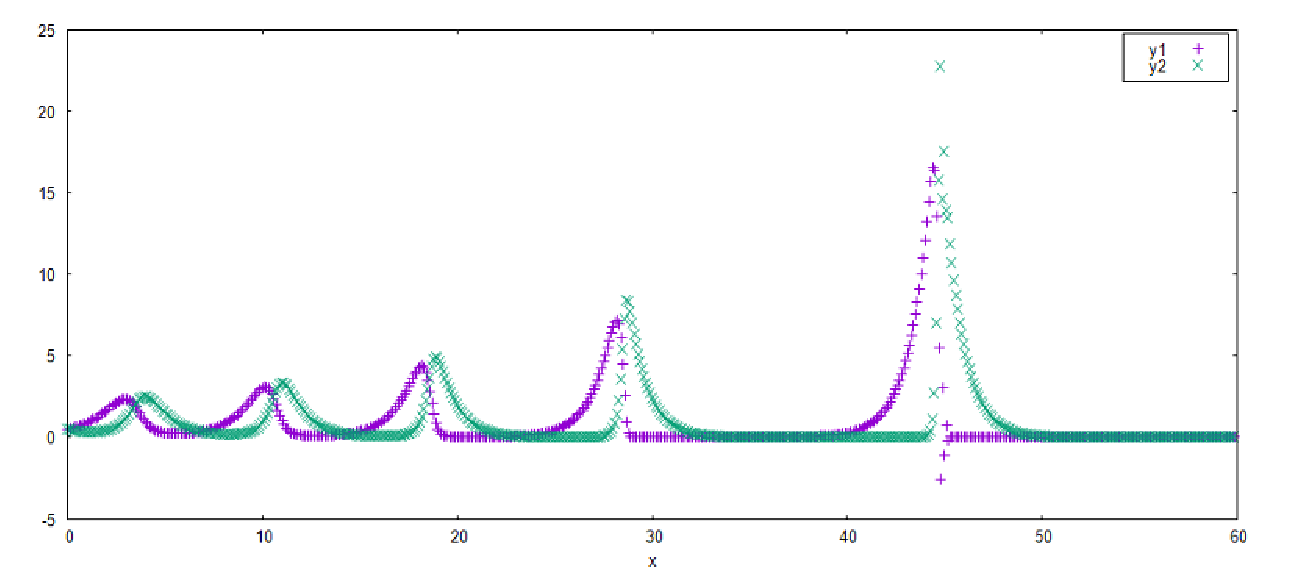
\includegraphics[scale=0.7]{./img/kadai5.eps}
\caption{生存競争モデル}
\label{graph_kadai5}
\end{figure}

生存競争モデルであるため$y_1$を被食者、$y_2$を捕食者として考えると、次のような循環があることがわかる.

\begin{enumerate}
 \item 被食者が増える。
 \item 捕食者が増える。
 \item 捕食者に食べられて被食者が減る。
 \item 被食者が少なくなったため,捕食者が減る。
 \item 捕食者が減ったため、被食者がまた増えて(1)に戻る。
\end{enumerate}

次に、初期条件を$y_1(0)=10,y_2(0)=0$とし、パラメータ$a,b,c,d$を変更した場合について考える。
パラメータの値を$a=1,b=1,c=0.01,d=0.01$とした場合のグラフを図\ref{5-1}に、
$a=0.01,b=1,c=1,d=0.01$とした場合のグラフを図\ref{5-2}に、
$a=1,b=0.01,c=0.01,d=1$とした場合のグラフを図\ref{5-3}に、
$a=b=c=d=1$とした場合のグラフを図\ref{5-4}に示す。

\begin{figure}[H]
\centering
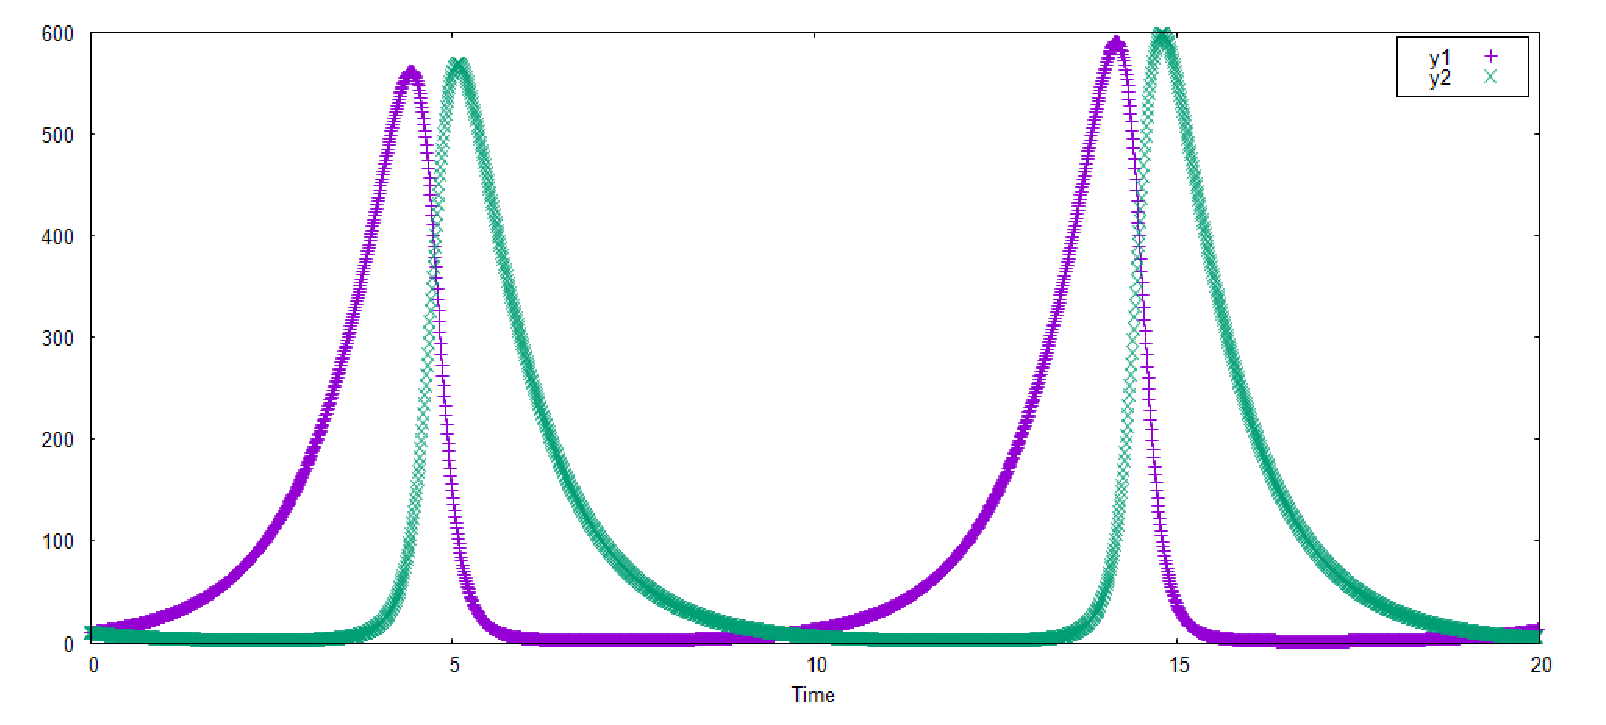
\includegraphics[scale=0.5]{./img/kadai5_1.eps}
\caption{$y_2<a/c,y_1<b/d$}
\label{5-1}
\end{figure}

\begin{figure}[H]
\centering
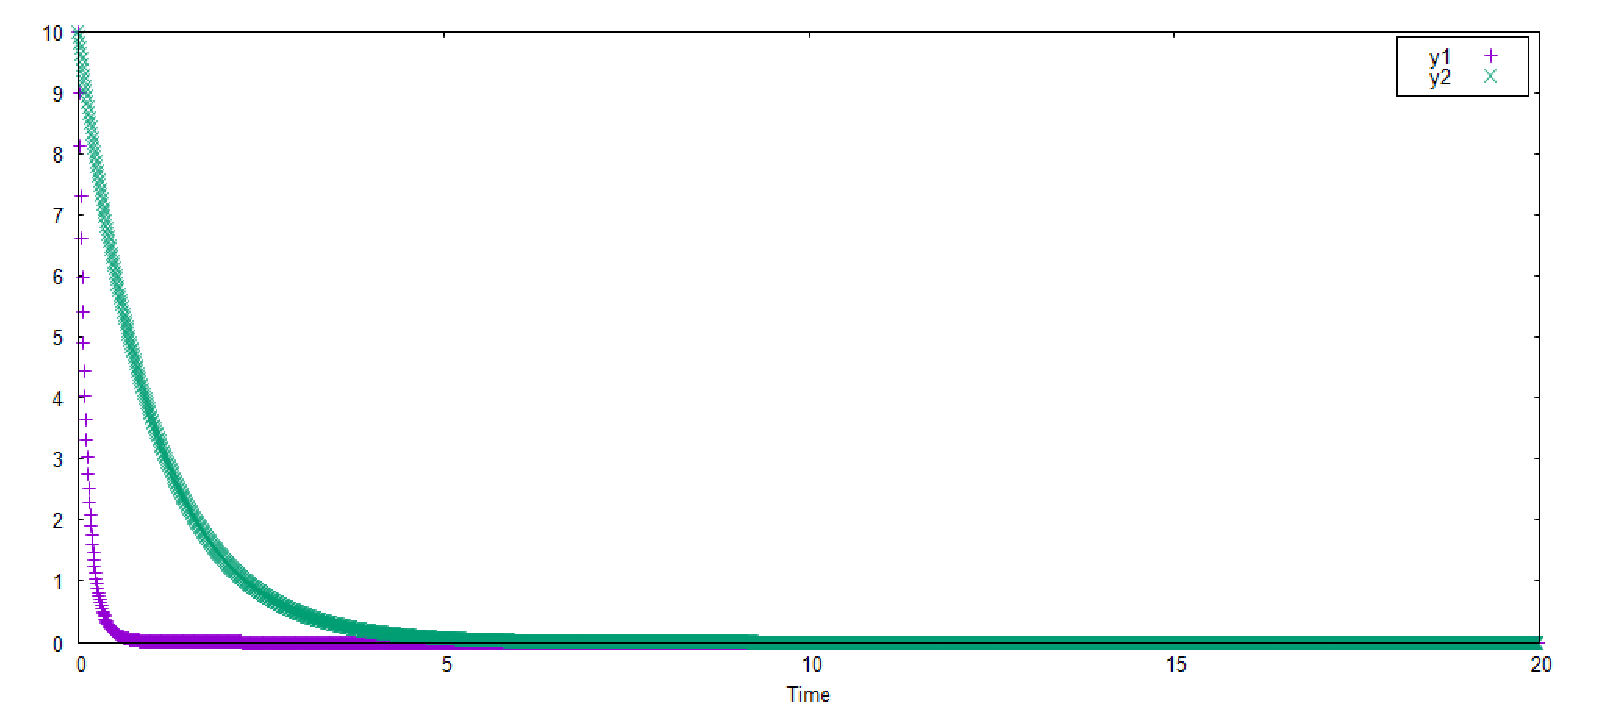
\includegraphics[scale=0.5]{./img/kadai5_2.eps}
\caption{$y_2>a/c,y_1<b/d$}
\label{5-2}
\end{figure}

\begin{figure}[H]
\centering
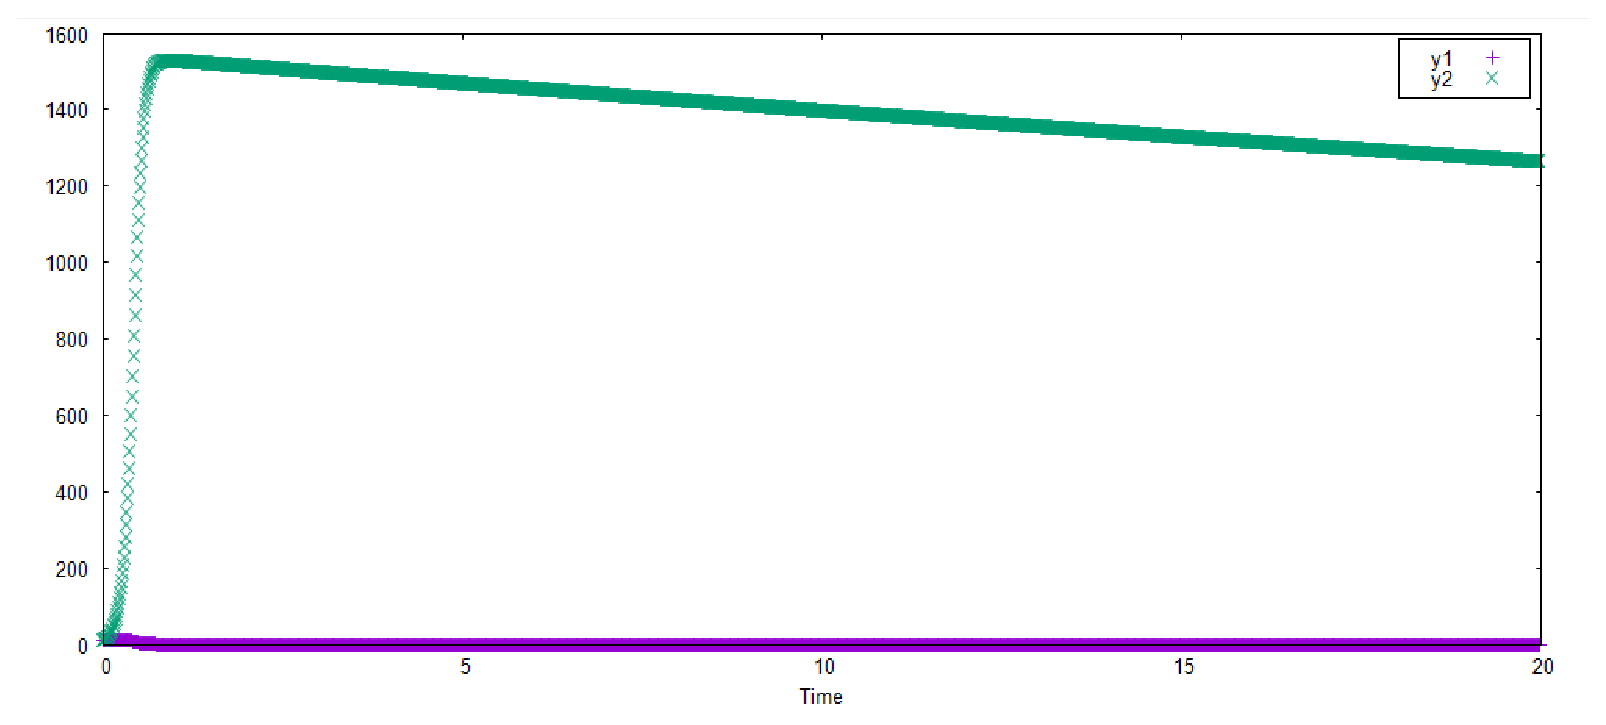
\includegraphics[scale=0.5]{./img/kadai5_3.eps}
\caption{$y_2<a/c,y_1>b/d$}
\label{5-3}
\end{figure}

\begin{figure}[H]
\centering
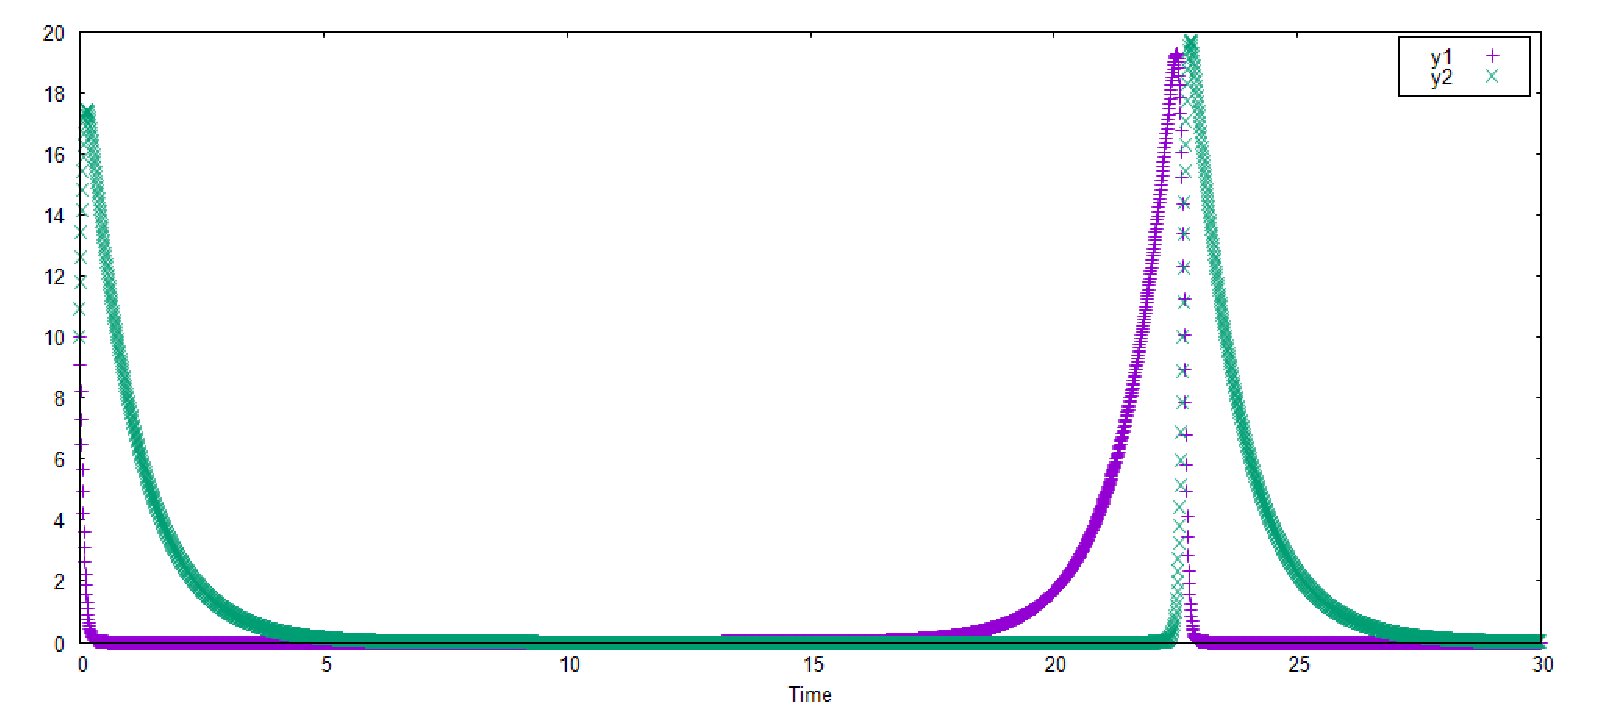
\includegraphics[scale=0.5]{./img/kadai5_4.eps}
\caption{$y_2>a/c,y_1>b/d$}
\label{5-4}
\end{figure}

図\ref{5-1}--\ref{5-4}と式(\ref{223759_6Jan19})より、パラメータ$a,b,c,d$には次のような意味があると考えられる.

\begin{itemize}
  \item $a$$\cdots$被食者の増えやすさ
  \item $b$$\cdots$捕食者の減りやすさ
  \item $c$$\cdots$捕食者の数と比例した被食者の減りやすさ
  \item $d$$\cdots$被食者の数と比例した捕食者の増えやすさ
\end{itemize}

図\ref{5-1}, \ref{5-4}では各パラメータのバランスが取れているため、前述した箇条書きのような循環が起こっている。
その一方で図\ref{5-2}, \ref{5-3}ではパラメータ同士のバランスが取れていないため、被食者の数が多くなり、
最終的にはどちらも絶滅してしまう。
図\ref{5-2}では$a$が小さく、$c$が大きいため、被食者が増えにくく減りやすくなる。
捕食者はパラメータ上では減りにくく増えにくいが、被食者が減りやすい状態においては捕食者も減りやすくなってしまう。
図\ref{5-3}では$b$が小さく$d$が大きいため、捕食者が増えやすく減りにくくなる。
被食者の数もパラメータ上では増やすく減りにくいので捕食者が一気に増加するが、被食者が減りすぎて捕食者は少しずつ少なくなっていく。
図\ref{5-2}とは異なり、捕食者が少しづつ減っているのはパラメータ$b$により減りにくくなっているためだと考えられる。


\section{課題7 : ニュートンの運動方程式}
式(\ref{newton1})に示す、ニュートンの運動方程式の高階微分方程式をオイラー法で解くプログラムを作成する。

\begin{eqnarray}
  \begin{cases}
mv'=-ky-lv&\\
y'= v&
 \label{newton1}
  \end{cases}\label{newton1}
\end{eqnarray}

\subsection{プログラムリスト}
課題7のプログラムリストをリスト\ref{lst:kadai7}に示す。

\lstinputlisting[style=C,caption=課題7のプログラム,label=lst:kadai7]{code/kadai07-2.c}

\subsection{実行結果}
課題7の実行結果をリスト\ref{lst:kekka7}に示す。

\begin{lstlisting}[style=text,caption=課題7の実行結果,label=lst:kekka7]
i =  0, t = 0.0000000000000000, y = 10.0000000000000000, v = 0.0000000000000000
i =  1, t = 0.0100000000000000, y = 10.0000000000000000, v = -0.1000000000000000
i =  2, t = 0.0200000000000000, y = 9.9990000000000006, v = -0.2000000000000000
i =  3, t = 0.0300000000000000, y = 9.9969999999999999, v = -0.2999900000000000
i =  4, t = 0.0400000000000000, y = 9.9940000999999992, v = -0.3999600000000000
i =  5, t = 0.0500000000000000, y = 9.9900004999999990, v = -0.4999000010000000
i =  6, t = 0.0600000000000000, y = 9.9850014999899983, v = -0.5998000060000001
i =  7, t = 0.0700000000000000, y = 9.9790034999299984, v = -0.6996500209999000
i =  8, t = 0.0800000000000000, y = 9.9720069997199996, v = -0.7994400559992000
i =  9, t = 0.0900000000000000, y = 9.9640125991600073, v = -0.8991601259963999
i = 10, t = 0.1000000000000000, y = 9.9550209979000428, v = -0.9988002519880000
i = 11, t = 0.1100000000000000, y = 9.9450329953801635, v = -1.0983504619670004
i = 12, t = 0.1200000000000000, y = 9.9340494907604935, v = -1.1978007919208020
i = 13, t = 0.1300000000000000, y = 9.9220714828412859, v = -1.2971412868284069
i = 14, t = 0.1400000000000000, y = 9.9091000699730021, v = -1.3963620016568197
i = 15, t = 0.1500000000000000, y = 9.8951364499564338, v = -1.4954530023565498
i = 16, t = 0.1600000000000000, y = 9.8801819199328680, v = -1.5944043668561141
i = 17, t = 0.1700000000000000, y = 9.8642378762643066, v = -1.6932061860554428
i = 18, t = 0.1800000000000000, y = 9.8473058144037520, v = -1.7918485648180860
i = 19, t = 0.1900000000000000, y = 9.8293873287555709, v = -1.8903216229621236
i = 20, t = 0.2000000000000000, y = 9.8104841125259501, v = -1.9886154962496794
i = 21, t = 0.2100000000000000, y = 9.7905979575634525, v = -2.0867203373749388
i = 22, t = 0.2200000000000001, y = 9.7697307541897036, v = -2.1846263169505735
i = 23, t = 0.2300000000000001, y = 9.7478844910201978, v = -2.2823236244924705
i = 24, t = 0.2400000000000001, y = 9.7250612547752731, v = -2.3798024694026725
i = 25, t = 0.2500000000000001, y = 9.7012632300812456, v = -2.4770530819504253
i = 26, t = 0.2600000000000001, y = 9.6764926992617415, v = -2.5740657142512378
i = 27, t = 0.2700000000000001, y = 9.6507520421192297, v = -2.6708306412438554
i = 28, t = 0.2800000000000001, y = 9.6240437357067918, v = -2.7673381616650476
i = 29, t = 0.2900000000000001, y = 9.5963703540901406, v = -2.8635785990221154
i = 30, t = 0.3000000000000001, y = 9.5677345680999188, v = -2.9595423025630168
i = 31, t = 0.3100000000000001, y = 9.5381391450742878, v = -3.0552196482440159
i = 32, t = 0.3200000000000001, y = 9.5075869485918485, v = -3.1506010396947590
i = 33, t = 0.3300000000000001, y = 9.4760809381949009, v = -3.2456769091806774
i = 34, t = 0.3400000000000001, y = 9.4436241691030940, v = -3.3404377185626264
i = 35, t = 0.3500000000000001, y = 9.4102197919174682, v = -3.4348739602536575
i = 36, t = 0.3600000000000002, y = 9.3758710523149311, v = -3.5289761581728323
i = 37, t = 0.3700000000000002, y = 9.3405812907332031, v = -3.6227348686959817
i = 38, t = 0.3800000000000002, y = 9.3043539420462427, v = -3.7161406816033136
i = 39, t = 0.3900000000000002, y = 9.2671925352302100, v = -3.8091842210237759
i = 40, t = 0.4000000000000002, y = 9.2291006930199728, v = -3.9018561463760779
i = 41, t = 0.4100000000000002, y = 9.1900821315562116, v = -3.9941471533062778
i = 42, t = 0.4200000000000002, y = 9.1501406600231494, v = -4.0860479746218399
i = 43, t = 0.4300000000000002, y = 9.1092801802769312, v = -4.1775493812220716
i = 44, t = 0.4400000000000002, y = 9.0675046864647104, v = -4.2686421830248413
i = 45, t = 0.4500000000000002, y = 9.0248182646344617, v = -4.3593172298894887
i = 46, t = 0.4600000000000002, y = 8.9812250923355670, v = -4.4495654125358337
i = 47, t = 0.4700000000000003, y = 8.9367294382102092, v = -4.5393776634591898
i = 48, t = 0.4800000000000003, y = 8.8913356615756172, v = -4.6287449578412918
i = 49, t = 0.4900000000000003, y = 8.8450482119972040, v = -4.7176583144570481
i = 50, t = 0.5000000000000002, y = 8.7978716288526329, v = -4.8061087965770204
i = 51, t = 0.5100000000000002, y = 8.7498105408868625, v = -4.8940875128655463
i = 52, t = 0.5200000000000002, y = 8.7008696657582068, v = -4.9815856182744147
i = 53, t = 0.5300000000000002, y = 8.6510538095754619, v = -5.0685943149319970
i = 54, t = 0.5400000000000003, y = 8.6003678664261418, v = -5.1551048530277512
i = 55, t = 0.5500000000000003, y = 8.5488168178958635, v = -5.2411085316920127
i = 56, t = 0.5600000000000003, y = 8.4964057325789426, v = -5.3265966998709713
i = 57, t = 0.5700000000000003, y = 8.4431397655802325, v = -5.4115607571967610
i = 58, t = 0.5800000000000003, y = 8.3890241580082652, v = -5.4959921548525630
i = 59, t = 0.5900000000000003, y = 8.3340642364597404, v = -5.5798823964326454
i = 60, t = 0.6000000000000003, y = 8.2782654124954131, v = -5.6632230387972431
i = 61, t = 0.6100000000000003, y = 8.2216331821074409, v = -5.7460056929221972
i = 62, t = 0.6200000000000003, y = 8.1641731251782197, v = -5.8282220247432717
i = 63, t = 0.6300000000000003, y = 8.1058909049307868, v = -5.9098637559950538
i = 64, t = 0.6400000000000003, y = 8.0467922673708365, v = -5.9909226650443612
i = 65, t = 0.6500000000000004, y = 7.9868830407203930, v = -6.0713905877180698
i = 66, t = 0.6600000000000004, y = 7.9261691348432119, v = -6.1512594181252735
i = 67, t = 0.6700000000000004, y = 7.8646565406619589, v = -6.2305211094737061
i = 68, t = 0.6800000000000004, y = 7.8023513295672222, v = -6.3091676748803254
i = 69, t = 0.6900000000000004, y = 7.7392596528184185, v = -6.3871911881759980
i = 70, t = 0.7000000000000004, y = 7.6753877409366584, v = -6.4645837847041818
i = 71, t = 0.7100000000000004, y = 7.6107419030896164, v = -6.5413376621135484
i = 72, t = 0.7200000000000004, y = 7.5453285264684808, v = -6.6174450811444450
i = 73, t = 0.7300000000000004, y = 7.4791540756570365, v = -6.6928983664091302
i = 74, t = 0.7400000000000004, y = 7.4122250919929451, v = -6.7676899071657006
i = 75, t = 0.7500000000000004, y = 7.3445481929212884, v = -6.8418121580856299
i = 76, t = 0.7600000000000005, y = 7.2761300713404324, v = -6.9152576400148424
i = 77, t = 0.7700000000000005, y = 7.2069774949402836, v = -6.9880189407282467
i = 78, t = 0.7800000000000005, y = 7.1370973055330014, v = -7.0600887156776500
i = 79, t = 0.7900000000000005, y = 7.0664964183762251, v = -7.1314596887329795
i = 80, t = 0.8000000000000005, y = 6.9951818214888952, v = -7.2021246529167415
i = 81, t = 0.8100000000000005, y = 6.9231605749597280, v = -7.2720764711316308
i = 82, t = 0.8200000000000005, y = 6.8504398102484121, v = -7.3413080768812282
i = 83, t = 0.8300000000000005, y = 6.7770267294795996, v = -7.4098124749837124
i = 84, t = 0.8400000000000005, y = 6.7029286047297623, v = -7.4775827422785088
i = 85, t = 0.8500000000000005, y = 6.6281527773069771, v = -7.5446120283258065
i = 86, t = 0.8600000000000005, y = 6.5527066570237187, v = -7.6108935560988762
i = 87, t = 0.8700000000000006, y = 6.4765977214627295, v = -7.6764206226691130
i = 88, t = 0.8800000000000006, y = 6.3998335152360379, v = -7.7411865998837399
i = 89, t = 0.8900000000000006, y = 6.3224216492372003, v = -7.8051849350361007
i = 90, t = 0.9000000000000006, y = 6.2443697998868393, v = -7.8684091515284731
i = 91, t = 0.9100000000000006, y = 6.1656857083715542, v = -7.9308528495273416
i = 92, t = 0.9200000000000006, y = 6.0863771798762807, v = -7.9925097066110569
i = 93, t = 0.9300000000000006, y = 6.0064520828101697, v = -8.0533734784098190
i = 94, t = 0.9400000000000006, y = 5.9259183480260713, v = -8.1134379992379202
i = 95, t = 0.9500000000000006, y = 5.8447839680336919, v = -8.1726971827181814
i = 96, t = 0.9600000000000006, y = 5.7630569962065099, v = -8.2311450223985183
i = 97, t = 0.9700000000000006, y = 5.6807455459825249, v = -8.2887755923605830
i = 98, t = 0.9800000000000006, y = 5.5978577900589190, v = -8.3455830478204085
i = 99, t = 0.9900000000000007, y = 5.5144019595807148, v = -8.4015616257209977
i = 100, t = 1.0000000000000007, y = 5.4303863433235051, v = -8.4567056453168057
\end{lstlisting}

\subsection{考察}
実行結果をグラフにプロットしたものを図\ref{101837_6Jan19}に示す。
図\ref{101837_6Jan19}は$l=0$であるため、単振動になっている。
次に、初期条件$k, l$を変更した場合のグラフを図\ref{mkl113}, \ref{mkl131}に示す。
3つのグラフから、ばね定数を示す$k$が$y, v$の振動のしやすさに、摩擦係数の$l$が振動のしにくさを表していることが分かる。
そのため図\ref{mkl113}は$l$が大きく、振動が止まっている。
図\ref{mkl131}は$k$が大きいため図\ref{mkl113}よりは振動するが、$l=1$であるため振動が止まる。

\begin{figure}[H]
\centering
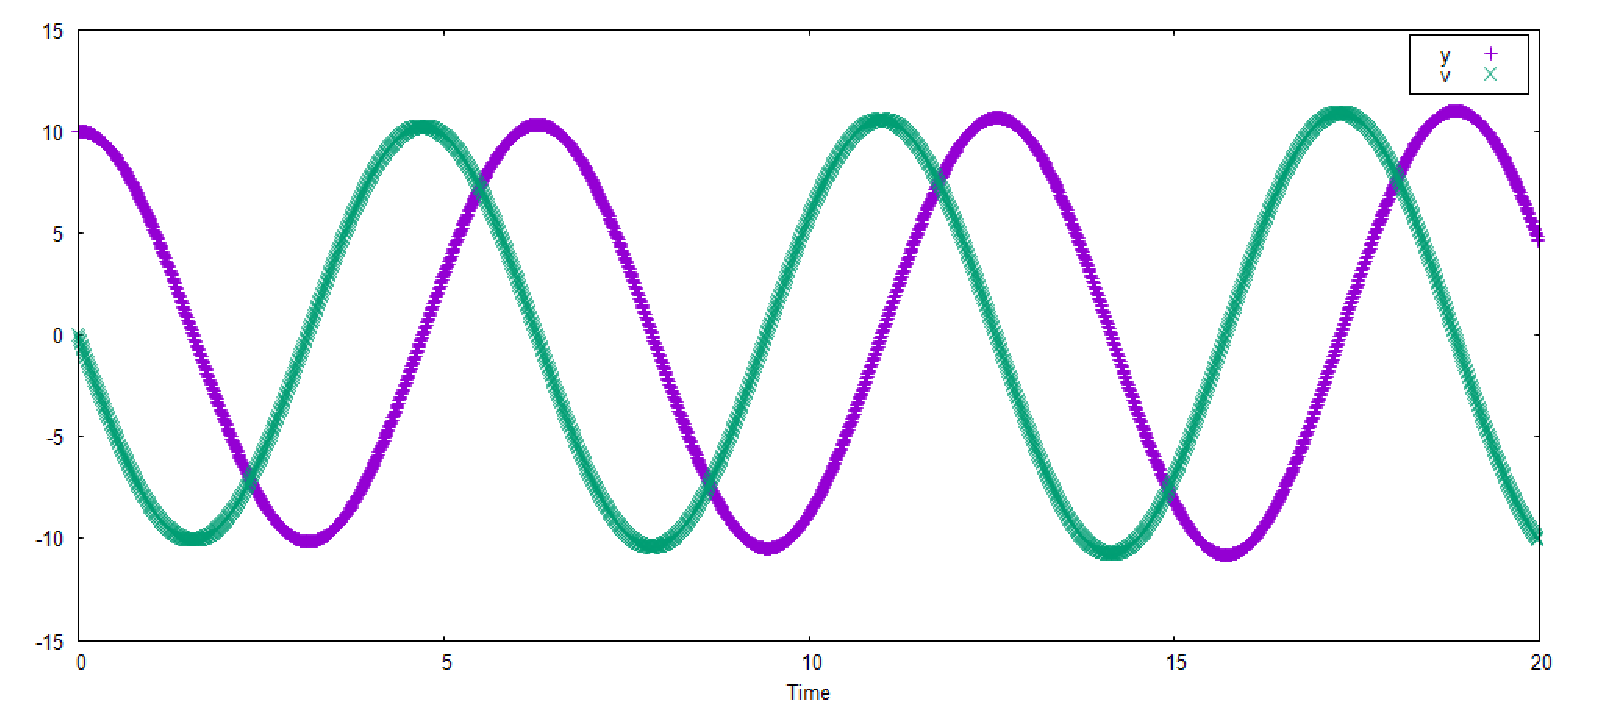
\includegraphics[scale=0.5]{./img/kadai6_1mkl_110.eps}
\caption{初期条件$m=1,k=1,l=0$}
\label{101837_6Jan19}
\end{figure}

\begin{figure}[H]
\centering
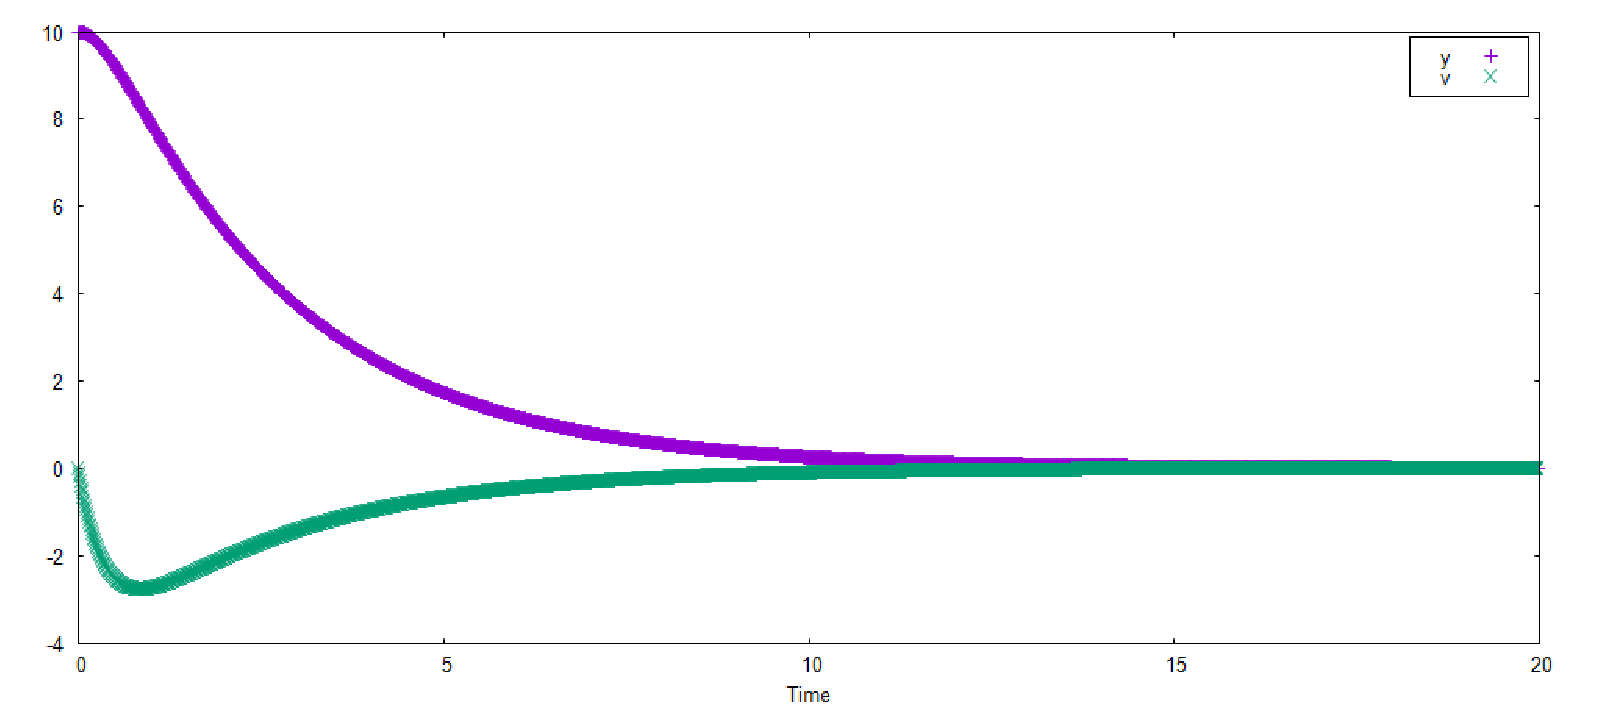
\includegraphics[scale=0.5]{./img/kadai6_2mkl_113.eps}
\caption{初期条件$k=1,l=3$}
\label{mkl113}
\end{figure}

\begin{figure}[H]
\centering
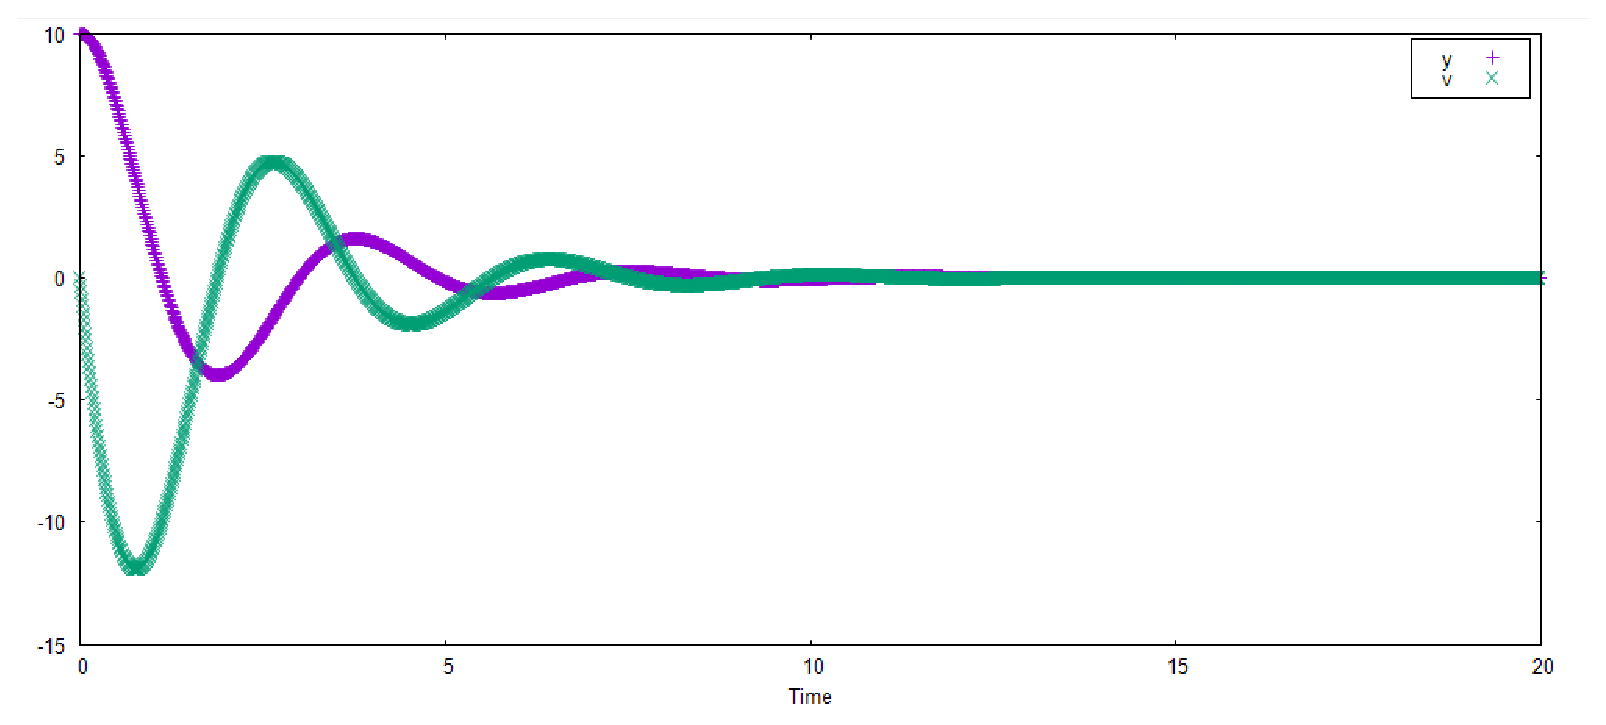
\includegraphics[scale=0.5]{./img/kadai6_3mkl_131.eps}
\caption{初期条件$k=3,l=1$}
\label{mkl131}
\end{figure}


\section{課題8 : RLC共振回路}
式(\ref{eq:kadai8})に示す、RLC共振回路の微分方程式をホイン法で解くプログラムを作成する。

\begin{equation}
  \frac{dV}{dt^2}+\frac{R}{L}\frac{dC}{dt}+\frac{V}{LC}=0
  \label{eq:kadai8}
\end{equation}

\subsection{プログラムリスト}
課題8のプログラムリストをリスト\ref{lst:kadai8}に示す。

\lstinputlisting[style=C,caption=課題8のプログラム,label=lst:kadai8]{code/kadai08-2.c}

\subsection{実行結果}
課題8の実行結果をリスト\ref{lst:kekka8}に示す。

\begin{lstlisting}[style=text,caption=課題8の実行結果,label=lst:kekka8]
i =  0, t = 0.0000000000000000, y = 10.0000000000000000, v = 0.0000000000000000
i =  1, t = 0.0100000000000000, y = 10.0000000000000000, v = -0.0333333333333333
i =  2, t = 0.0200000000000000, y = 9.9996650000000002, v = -0.0666333500000000
i =  3, t = 0.0300000000000000, y = 9.9989953348325002, v = -0.0998989671916750
i =  4, t = 0.0400000000000000, y = 9.9979913502122244, v = -0.1331291042978505
i =  5, t = 0.0500000000000000, y = 9.9966534027140312, v = -0.1663226829398952
i =  6, t = 0.0600000000000000, y = 9.9949818597504851, v = -0.1994786270050057
i =  7, t = 0.0700000000000000, y = 9.9929770995490852, v = -0.2325958626800496
i =  8, t = 0.0800000000000000, y = 9.9906395111291513, v = -0.2656733184852986
i =  9, t = 0.0900000000000000, y = 9.9879694942783743, v = -0.2987099253080512
i = 10, t = 0.1000000000000000, y = 9.9849674595290292, v = -0.3317046164361432
i = 11, t = 0.1100000000000000, y = 9.9816338281338464, v = -0.3646563275913462
i = 12, t = 0.1200000000000000, y = 9.9779690320415533, v = -0.3975639969626513
i = 13, t = 0.1300000000000000, y = 9.9739735138720782, v = -0.4304265652394389
i = 14, t = 0.1400000000000000, y = 9.9696477268914219, v = -0.4632429756445325
i = 15, t = 0.1500000000000000, y = 9.9649921349861952, v = -0.4960121739671358
i = 16, t = 0.1600000000000000, y = 9.9600072126378247, v = -0.5287331085956513
i = 17, t = 0.1700000000000000, y = 9.9546934448964386, v = -0.5614047305503815
i = 18, t = 0.1800000000000000, y = 9.9490513273544074, v = -0.5940259935161097
i = 19, t = 0.1900000000000000, y = 9.9430813661195714, v = -0.6265958538745595
i = 20, t = 0.2000000000000000, y = 9.9367840777881327, v = -0.6591132707367336
i = 21, t = 0.2100000000000000, y = 9.9301599894172288, v = -0.6915772059751297
i = 22, t = 0.2200000000000001, y = 9.9232096384971786, v = -0.7239866242558326
i = 23, t = 0.2300000000000001, y = 9.9159335729234073, v = -0.7563404930704820
i = 24, t = 0.2400000000000001, y = 9.9083323509680490, v = -0.7886377827681146
i = 25, t = 0.2500000000000001, y = 9.9004065412512290, v = -0.8208774665868798
i = 26, t = 0.2600000000000001, y = 9.8921567227120306, v = -0.8530585206856282
i = 27, t = 0.2700000000000001, y = 9.8835834845791393, v = -0.8851799241753718
i = 28, t = 0.2800000000000001, y = 9.8746874263411772, v = -0.9172406591506147
i = 29, t = 0.2900000000000001, y = 9.8654691577167135, v = -0.9492397107205537
i = 30, t = 0.3000000000000001, y = 9.8559292986239715, v = -0.9811760670401480
i = 31, t = 0.3100000000000001, y = 9.8460684791502189, v = -1.0130487193410569
i = 32, t = 0.3200000000000001, y = 9.8358873395208413, v = -1.0448566619624444
i = 33, t = 0.3300000000000001, y = 9.8253865300681191, v = -1.0765988923816499
i = 34, t = 0.3400000000000001, y = 9.8145667111996833, v = -1.1082744112447247
i = 35, t = 0.3500000000000001, y = 9.8034285533666736, v = -1.1398822223968326
i = 36, t = 0.3600000000000002, y = 9.7919727370315854, v = -1.1714213329125136
i = 37, t = 0.3700000000000002, y = 9.7801999526358152, v = -1.2028907531258111
i = 38, t = 0.3800000000000002, y = 9.7681109005669011, v = -1.2342894966602602
i = 39, t = 0.3900000000000002, y = 9.7557062911254651, v = -1.2656165804587369
i = 40, t = 0.4000000000000002, y = 9.7429868444918544, v = -1.2968710248131681
i = 41, t = 0.4100000000000002, y = 9.7299532906924817, v = -1.3280518533940993
i = 42, t = 0.4200000000000002, y = 9.7166063695658718, v = -1.3591580932801224
i = 43, t = 0.4300000000000002, y = 9.7029468307284059, v = -1.3901887749871591
i = 44, t = 0.4400000000000002, y = 9.6889754335397846, v = -1.4211429324976028
i = 45, t = 0.4500000000000002, y = 9.6746929470681842, v = -1.4520196032893149
i = 46, t = 0.4600000000000002, y = 9.6601001500551273, v = -1.4828178283644760
i = 47, t = 0.4700000000000003, y = 9.6451978308800648, v = -1.5135366522782927
i = 48, t = 0.4800000000000003, y = 9.6299867875246683, v = -1.5441751231675560
i = 49, t = 0.4900000000000003, y = 9.6144678275368349, v = -1.5747322927790530
i = 50, t = 0.5000000000000002, y = 9.5986417679944047, v = -1.6052072164978306
i = 51, t = 0.5100000000000002, y = 9.5825094354686016, v = -1.6355989533753090
i = 52, t = 0.5200000000000002, y = 9.5660716659871792, v = -1.6659065661572465
i = 53, t = 0.5300000000000002, y = 9.5493293049972987, v = -1.6961291213115530
i = 54, t = 0.5400000000000003, y = 9.5322832073281170, v = -1.7262656890559516
i = 55, t = 0.5500000000000003, y = 9.5149342371531045, v = -1.7563153433854883
i = 56, t = 0.5600000000000003, y = 9.4972832679520796, v = -1.7862771620998896
i = 57, t = 0.5700000000000003, y = 9.4793311824729756, v = -1.8161502268307645
i = 58, t = 0.5800000000000003, y = 9.4610788726933261, v = -1.8459336230686529
i = 59, t = 0.5900000000000003, y = 9.4425272397814854, v = -1.8756264401899192
i = 60, t = 0.6000000000000003, y = 9.4236771940575768, v = -1.9052277714834880
i = 61, t = 0.6100000000000003, y = 9.4045296549541675, v = -1.9347367141774254
i = 62, t = 0.6200000000000003, y = 9.3850855509766848, v = -1.9641523694653606
i = 63, t = 0.6300000000000003, y = 9.3653458196635579, v = -1.9934738425327507
i = 64, t = 0.6400000000000003, y = 9.3453114075461041, v = -2.0227002425829852
i = 65, t = 0.6500000000000004, y = 9.3249832701081452, v = -2.0518306828633315
i = 66, t = 0.6600000000000004, y = 9.3043623717453681, v = -2.0808642806907200
i = 67, t = 0.6700000000000004, y = 9.2834496857244257, v = -2.1098001574773679
i = 68, t = 0.6800000000000004, y = 9.2622461941417775, v = -2.1386374387562412
i = 69, t = 0.6900000000000004, y = 9.2407528878822767, v = -2.1673752542063536
i = 70, t = 0.7000000000000004, y = 9.2189707665775025, v = -2.1960127376779019
i = 71, t = 0.7100000000000004, y = 9.1969008385638400, v = -2.2245490272172401
i = 72, t = 0.7200000000000004, y = 9.1745441208403076, v = -2.2529832650916850
i = 73, t = 0.7300000000000004, y = 9.1519016390261356, v = -2.2813145978141587
i = 74, t = 0.7400000000000004, y = 9.1289744273181039, v = -2.3095421761676653
i = 75, t = 0.7500000000000004, y = 9.1057635284476195, v = -2.3376651552296006
i = 76, t = 0.7600000000000005, y = 9.0822699936375617, v = -2.3656826943958933
i = 77, t = 0.7700000000000005, y = 9.0584948825588825, v = -2.3935939574049803
i = 78, t = 0.7800000000000005, y = 9.0344392632869628, v = -2.4213981123616128
i = 79, t = 0.7900000000000005, y = 9.0101042122577280, v = -2.4490943317604916
i = 80, t = 0.8000000000000005, y = 8.9854908142235352, v = -2.4766817925097357
i = 81, t = 0.8100000000000005, y = 8.9606001622088129, v = -2.5041596759541771
i = 82, t = 0.8200000000000005, y = 8.9354333574654738, v = -2.5315271678984868
i = 83, t = 0.8300000000000005, y = 8.9099915094280941, v = -2.5587834586301281
i = 84, t = 0.8400000000000005, y = 8.8842757356688615, v = -2.5859277429421388
i = 85, t = 0.8500000000000005, y = 8.8582871618522923, v = -2.6129592201557381
i = 86, t = 0.8600000000000005, y = 8.8320269216897263, v = -2.6398770941427636
i = 87, t = 0.8700000000000006, y = 8.8054961568935912, v = -2.6666805733479308
i = 88, t = 0.8800000000000006, y = 8.7786960171314448, v = -2.6933688708109202
i = 89, t = 0.8900000000000006, y = 8.7516276599797944, v = -2.7199412041882876
i = 90, t = 0.9000000000000006, y = 8.7242922508777028, v = -2.7463967957752007
i = 91, t = 0.9100000000000006, y = 8.6966909630801617, v = -2.7727348725269976
i = 92, t = 0.9200000000000006, y = 8.6688249776112656, v = -2.7989546660805691
i = 93, t = 0.9300000000000006, y = 8.6406954832171561, v = -2.8250554127755629
i = 94, t = 0.9400000000000006, y = 8.6123036763187617, v = -2.8510363536754122
i = 95, t = 0.9500000000000006, y = 8.5836507609643231, v = -2.8768967345881822
i = 96, t = 0.9600000000000006, y = 8.5547379487817121, v = -2.9026358060872406
i = 97, t = 0.9700000000000006, y = 8.5255664589305358, v = -2.9282528235317473
i = 98, t = 0.9800000000000006, y = 8.4961375180540415, v = -2.9537470470869645
i = 99, t = 0.9900000000000007, y = 8.4664523602308179, v = -2.9791177417443846
i = 100, t = 1.0000000000000007, y = 8.4365122269262862, v = -3.0043641773416803
\end{lstlisting}

\subsection{考察}
$R=0,3,6,9,2\sqrt{L/C}$の場合それぞれについてプロットしたグラフを図\ref{r0}--\ref{rsqr}に示す。
図\ref{r0}より刻み幅は0.01が減衰しない刻み幅であることがわかった。

\begin{figure}[H]
\centering
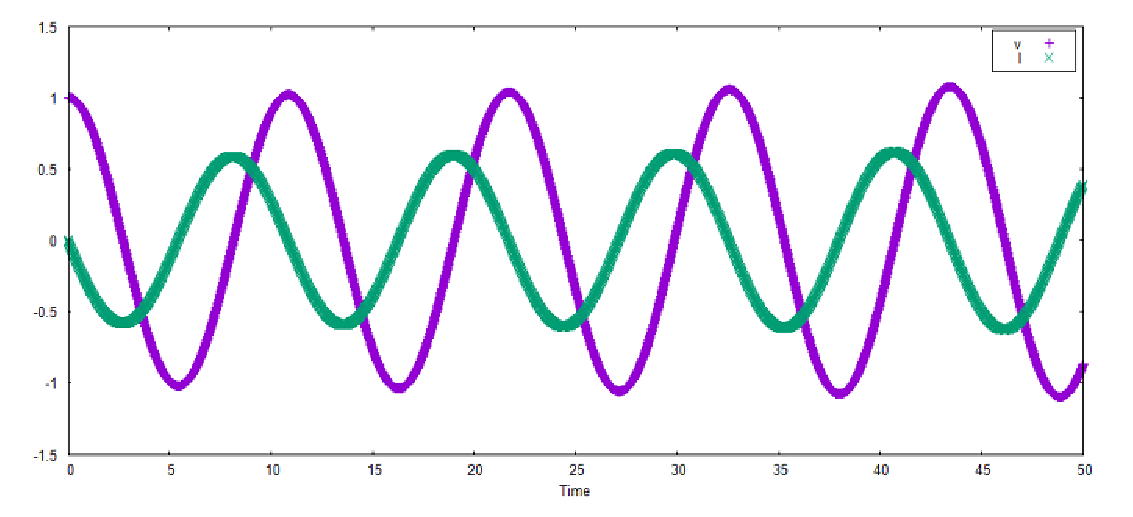
\includegraphics[scale=0.7]{./img/kadai7_R0.eps}
\caption{$R=0$}
\label{r0}
\end{figure}

\begin{figure}[H]
\centering
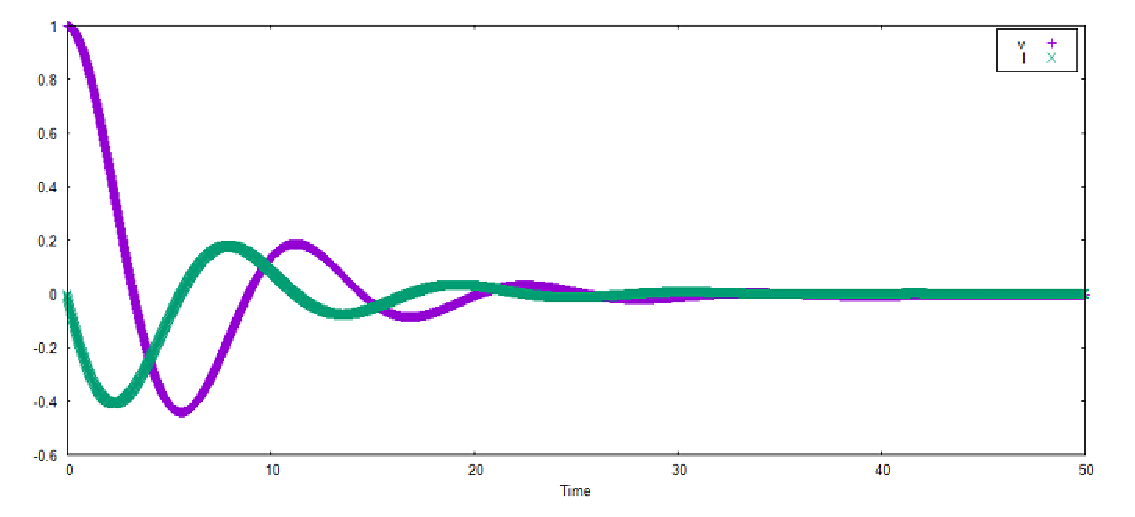
\includegraphics[scale=0.7]{./img/kadai7_R3.eps}
\caption{$R=3$}
\label{r3}
\end{figure}

\begin{figure}[H]
\centering
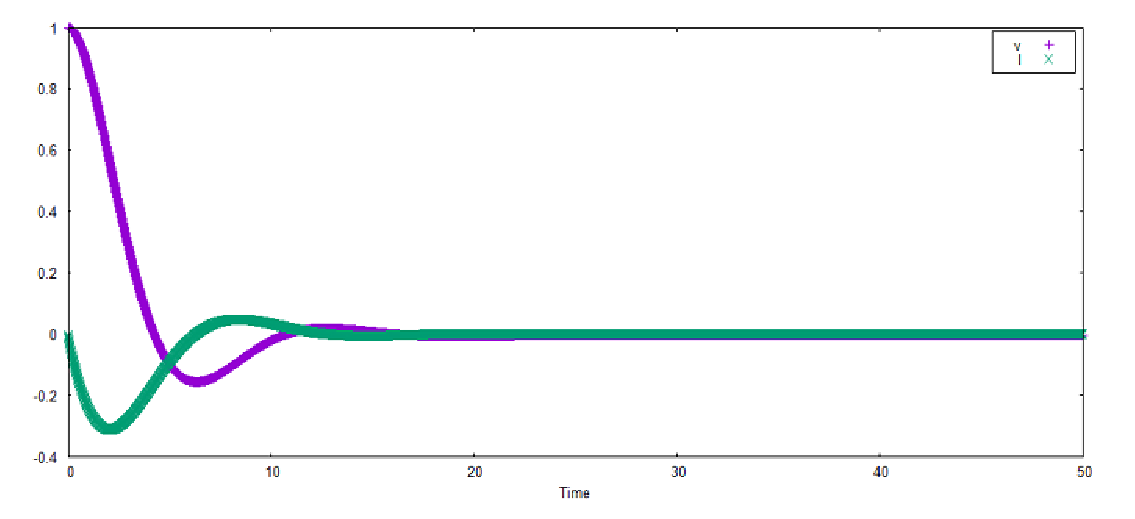
\includegraphics[scale=0.7]{./img/kadai7_R6.eps}
\caption{$R=6$}
\label{r6}
\end{figure}

\begin{figure}[H]
\centering
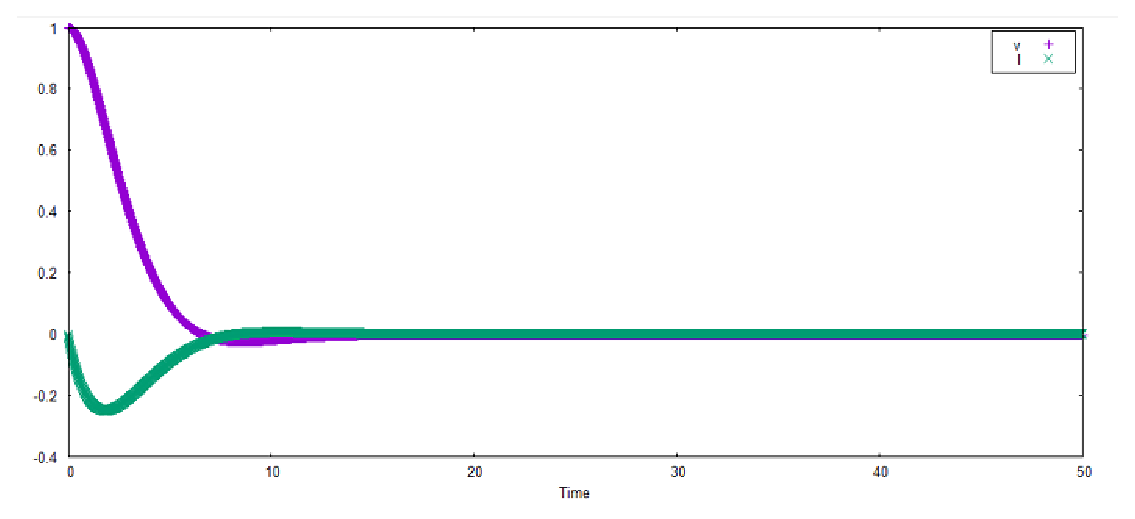
\includegraphics[scale=0.7]{./img/kadai7_R9.eps}
\caption{$R=9$}
\label{r9}
\end{figure}

\begin{figure}[H]
\centering
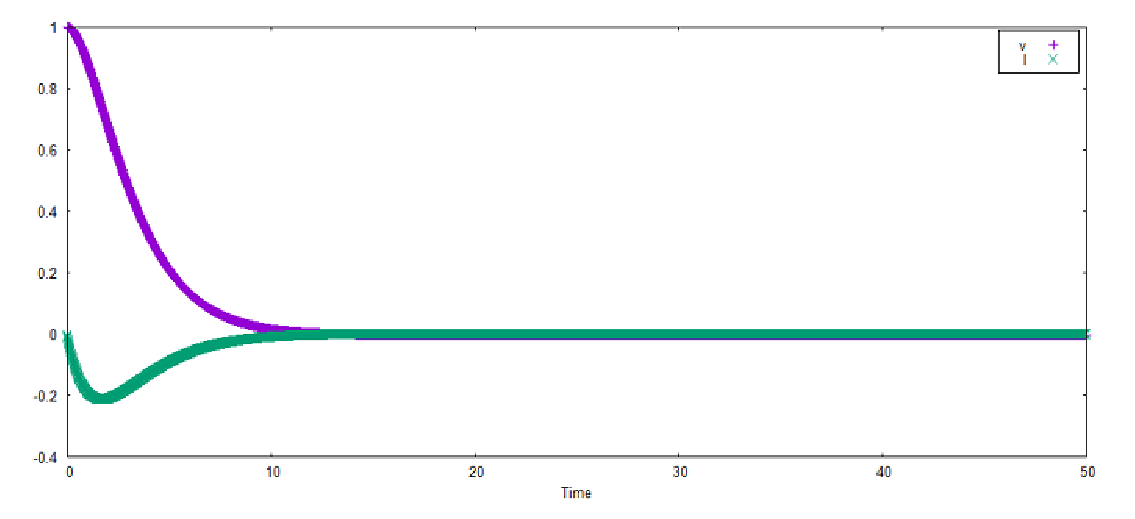
\includegraphics[scale=0.7]{./img/kadai7_sqr.eps}
\caption{$R=2\sqrt{L/C}$}
\label{rsqr}
\end{figure}

図\ref{r0}--\ref{rsqr}より、$R$が大きければ大きいほど振動が収まりやすくなっているため、
$R$は振動のしやすさに関連していることがわかる。
これは$R$が抵抗の値であり、$R$と$V$, $I$が反比例の関係にあるためだと考えられる。


\section{課題9 : ローレンツ力}
式(\ref{eq:kadai9-1}), (\ref{eq:kadai9-2})に示す、ローレンツ力についての連立微分方程式をホイン法で解くプログラムを作成する。

\begin{equation}
  \frac{d^2 x}{dt} = \frac{q}{m} v_y B_0 ,\, \frac{dx}{dt} = v_x
  \label{eq:kadai9-1}
\end{equation}

\begin{equation}
  \frac{d^2 y}{dt} = - \frac{q}{m} v_y B_0 ,\, \frac{dy}{dt} = v_y
  \label{eq:kadai9-2}
\end{equation}

\subsection{プログラムリスト}
課題9のプログラムリストをリスト\ref{lst:kadai9}に示す。

\lstinputlisting[style=C,caption=課題9のプログラム,label=lst:kadai9]{code/kadai09-2.c}

\subsection{実行結果}
課題9の実行結果をリスト\ref{lst:kekka9}に示す。

\begin{lstlisting}[style=text,caption=課題9の実行結果,label=lst:kekka9]
t = 0.00, x = 0.100000, y = 0.000000, vx = 1.000000, vy = 0.100000
t = 0.01, x = 0.110050, y = 0.001005, vx = 1.002020, vy = 0.080200
t = 0.02, x = 0.120120, y = 0.001811, vx = 1.003640, vy = 0.060360
t = 0.03, x = 0.130207, y = 0.002418, vx = 1.004859, vy = 0.040488
t = 0.04, x = 0.140306, y = 0.002825, vx = 1.005677, vy = 0.020592
t = 0.05, x = 0.150413, y = 0.003031, vx = 1.006093, vy = 0.000679
t = 0.06, x = 0.160524, y = 0.003038, vx = 1.006107, vy = -0.019241
t = 0.07, x = 0.170635, y = 0.002845, vx = 1.005718, vy = -0.039162
t = 0.08, x = 0.180743, y = 0.002451, vx = 1.004927, vy = -0.059075
t = 0.09, x = 0.190842, y = 0.001858, vx = 1.003734, vy = -0.078973
t = 0.10, x = 0.200930, y = 0.001064, vx = 1.002139, vy = -0.098847
t = 0.11, x = 0.211001, y = 0.000071, vx = 1.000142, vy = -0.118689
t = 0.12, x = 0.221053, y = -0.001122, vx = 0.997744, vy = -0.138492
t = 0.13, x = 0.231080, y = -0.002514, vx = 0.994947, vy = -0.158247
t = 0.14, x = 0.241079, y = -0.004105, vx = 0.991750, vy = -0.177947
t = 0.15, x = 0.251046, y = -0.005893, vx = 0.988156, vy = -0.197584
t = 0.16, x = 0.260977, y = -0.007879, vx = 0.984164, vy = -0.217150
t = 0.17, x = 0.270868, y = -0.010061, vx = 0.979778, vy = -0.236636
t = 0.18, x = 0.280715, y = -0.012439, vx = 0.974998, vy = -0.256036
t = 0.19, x = 0.290514, y = -0.015012, vx = 0.969826, vy = -0.275341
t = 0.20, x = 0.300261, y = -0.017779, vx = 0.964264, vy = -0.294543
t = 0.21, x = 0.309951, y = -0.020740, vx = 0.958314, vy = -0.313636
t = 0.22, x = 0.319582, y = -0.023892, vx = 0.951979, vy = -0.332610
t = 0.23, x = 0.329150, y = -0.027234, vx = 0.945260, vy = -0.351459
t = 0.24, x = 0.338650, y = -0.030767, vx = 0.938161, vy = -0.370175
t = 0.25, x = 0.348078, y = -0.034487, vx = 0.930683, vy = -0.388751
t = 0.26, x = 0.357432, y = -0.038394, vx = 0.922830, vy = -0.407179
t = 0.27, x = 0.366706, y = -0.042486, vx = 0.914605, vy = -0.425451
t = 0.28, x = 0.375898, y = -0.046762, vx = 0.906011, vy = -0.443560
t = 0.29, x = 0.385003, y = -0.051219, vx = 0.897051, vy = -0.461499
t = 0.30, x = 0.394019, y = -0.055858, vx = 0.887729, vy = -0.479260
t = 0.31, x = 0.402940, y = -0.060674, vx = 0.878048, vy = -0.496838
t = 0.32, x = 0.411765, y = -0.065667, vx = 0.868012, vy = -0.514223
t = 0.33, x = 0.420488, y = -0.070835, vx = 0.857625, vy = -0.531409
t = 0.34, x = 0.429107, y = -0.076176, vx = 0.846890, vy = -0.548390
t = 0.35, x = 0.437619, y = -0.081687, vx = 0.835813, vy = -0.565159
t = 0.36, x = 0.446018, y = -0.087367, vx = 0.824396, vy = -0.581708
t = 0.37, x = 0.454304, y = -0.093213, vx = 0.812646, vy = -0.598031
t = 0.38, x = 0.462471, y = -0.099223, vx = 0.800566, vy = -0.614121
t = 0.39, x = 0.470516, y = -0.105395, vx = 0.788160, vy = -0.629973
t = 0.40, x = 0.478437, y = -0.111727, vx = 0.775435, vy = -0.645578
t = 0.41, x = 0.486231, y = -0.118215, vx = 0.762394, vy = -0.660932
t = 0.42, x = 0.493893, y = -0.124857, vx = 0.749044, vy = -0.676027
t = 0.43, x = 0.501420, y = -0.131651, vx = 0.735388, vy = -0.690858
t = 0.44, x = 0.508811, y = -0.138594, vx = 0.721432, vy = -0.705419
t = 0.45, x = 0.516062, y = -0.145684, vx = 0.707183, vy = -0.719703
t = 0.46, x = 0.523169, y = -0.152917, vx = 0.692645, vy = -0.733706
t = 0.47, x = 0.530130, y = -0.160290, vx = 0.677824, vy = -0.747420
t = 0.48, x = 0.536942, y = -0.167802, vx = 0.662726, vy = -0.760841
t = 0.49, x = 0.543602, y = -0.175448, vx = 0.647357, vy = -0.773963
t = 0.50, x = 0.550108, y = -0.183227, vx = 0.631723, vy = -0.786780
t = 0.51, x = 0.556457, y = -0.191134, vx = 0.615830, vy = -0.799289
t = 0.52, x = 0.562646, y = -0.199167, vx = 0.599685, vy = -0.811482
t = 0.53, x = 0.568673, y = -0.207322, vx = 0.583293, vy = -0.823356
t = 0.54, x = 0.574535, y = -0.215597, vx = 0.566661, vy = -0.834905
t = 0.55, x = 0.580230, y = -0.223988, vx = 0.549796, vy = -0.846125
t = 0.56, x = 0.585755, y = -0.232491, vx = 0.532704, vy = -0.857011
t = 0.57, x = 0.591109, y = -0.241104, vx = 0.515392, vy = -0.867558
t = 0.58, x = 0.596289, y = -0.249823, vx = 0.497868, vy = -0.877763
t = 0.59, x = 0.601292, y = -0.258645, vx = 0.480137, vy = -0.887621
t = 0.60, x = 0.606118, y = -0.267565, vx = 0.462207, vy = -0.897128
t = 0.61, x = 0.610763, y = -0.276581, vx = 0.444085, vy = -0.906279
t = 0.62, x = 0.615226, y = -0.285690, vx = 0.425778, vy = -0.915072
t = 0.63, x = 0.619505, y = -0.294886, vx = 0.407294, vy = -0.923503
t = 0.64, x = 0.623598, y = -0.304167, vx = 0.388639, vy = -0.931567
t = 0.65, x = 0.627504, y = -0.313529, vx = 0.369821, vy = -0.939262
t = 0.66, x = 0.631221, y = -0.322969, vx = 0.350848, vy = -0.946585
t = 0.67, x = 0.634747, y = -0.332482, vx = 0.331727, vy = -0.953531
t = 0.68, x = 0.638081, y = -0.342065, vx = 0.312466, vy = -0.960100
t = 0.69, x = 0.641221, y = -0.351714, vx = 0.293072, vy = -0.966286
t = 0.70, x = 0.644166, y = -0.361425, vx = 0.273553, vy = -0.972089
t = 0.71, x = 0.646916, y = -0.371195, vx = 0.253917, vy = -0.977506
t = 0.72, x = 0.649468, y = -0.381019, vx = 0.234171, vy = -0.982533
t = 0.73, x = 0.651821, y = -0.390893, vx = 0.214324, vy = -0.987170
t = 0.74, x = 0.653975, y = -0.400814, vx = 0.194383, vy = -0.991413
t = 0.75, x = 0.655928, y = -0.410778, vx = 0.174357, vy = -0.995262
t = 0.76, x = 0.657681, y = -0.420780, vx = 0.154252, vy = -0.998714
t = 0.77, x = 0.659231, y = -0.430818, vx = 0.134078, vy = -1.001769
t = 0.78, x = 0.660578, y = -0.440885, vx = 0.113843, vy = -1.004423
t = 0.79, x = 0.661723, y = -0.450980, vx = 0.093553, vy = -1.006677
t = 0.80, x = 0.662663, y = -0.461097, vx = 0.073218, vy = -1.008530
t = 0.81, x = 0.663399, y = -0.471233, vx = 0.052846, vy = -1.009979
t = 0.82, x = 0.663930, y = -0.481383, vx = 0.032444, vy = -1.011026
t = 0.83, x = 0.664256, y = -0.491544, vx = 0.012022, vy = -1.011668
t = 0.84, x = 0.664377, y = -0.501711, vx = -0.008414, vy = -1.011906
t = 0.85, x = 0.664292, y = -0.511881, vx = -0.028855, vy = -1.011740
t = 0.86, x = 0.664002, y = -0.522049, vx = -0.049292, vy = -1.011168
t = 0.87, x = 0.663507, y = -0.532211, vx = -0.069717, vy = -1.010192
t = 0.88, x = 0.662806, y = -0.542363, vx = -0.090123, vy = -1.008812
t = 0.89, x = 0.661900, y = -0.552502, vx = -0.110501, vy = -1.007027
t = 0.90, x = 0.660790, y = -0.562622, vx = -0.130843, vy = -1.004840
t = 0.91, x = 0.659475, y = -0.572721, vx = -0.151141, vy = -1.002249
t = 0.92, x = 0.657956, y = -0.582794, vx = -0.171386, vy = -0.999256
t = 0.93, x = 0.656233, y = -0.592836, vx = -0.191571, vy = -0.995863
t = 0.94, x = 0.654308, y = -0.602845, vx = -0.211688, vy = -0.992070
t = 0.95, x = 0.652181, y = -0.612815, vx = -0.231728, vy = -0.987878
t = 0.96, x = 0.649852, y = -0.622743, vx = -0.251683, vy = -0.983290
t = 0.97, x = 0.647322, y = -0.632625, vx = -0.271545, vy = -0.978307
t = 0.98, x = 0.644593, y = -0.642457, vx = -0.291307, vy = -0.972930
t = 0.99, x = 0.641666, y = -0.652235, vx = -0.310960, vy = -0.967162
t = 1.00, x = 0.638541, y = -0.661955, vx = -0.330497, vy = -0.961005
\end{lstlisting}

\subsection{考察}
$q=m=1$, $B=1, 2, 10$のときの計算結果をプロットしたグラフを図\ref{8b1}--\ref{8b10}に示す。

\begin{figure}[H]
\centering
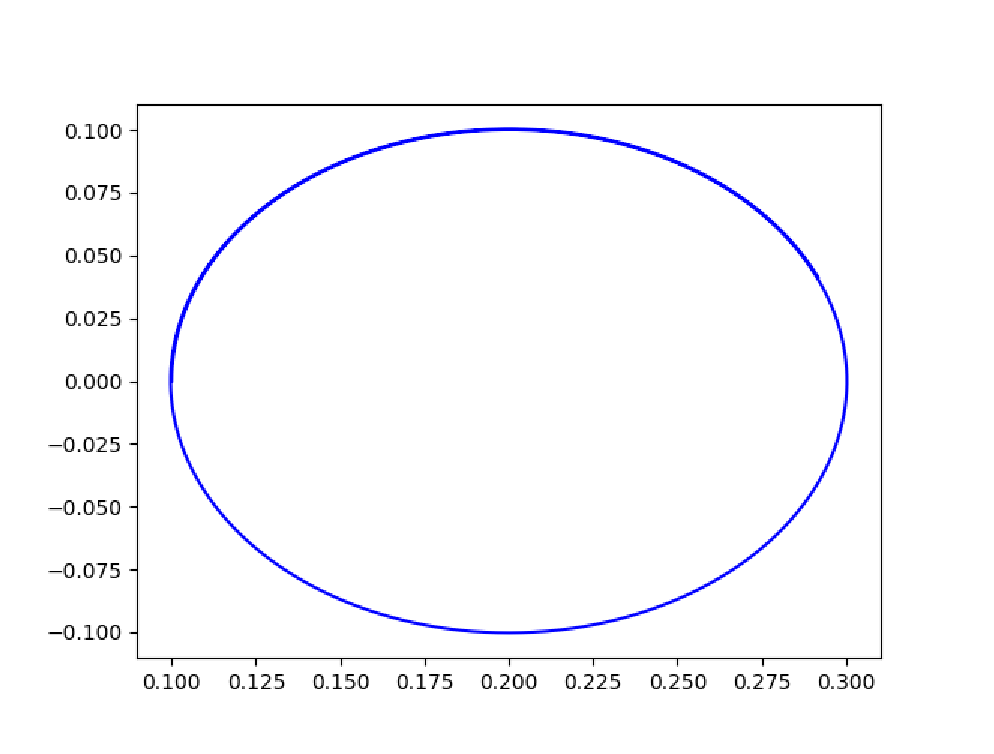
\includegraphics[scale=0.8]{./img/ka8_b1.eps}
\caption{$B=1$}
\label{8b1}
\end{figure}

\begin{figure}[H]
\centering
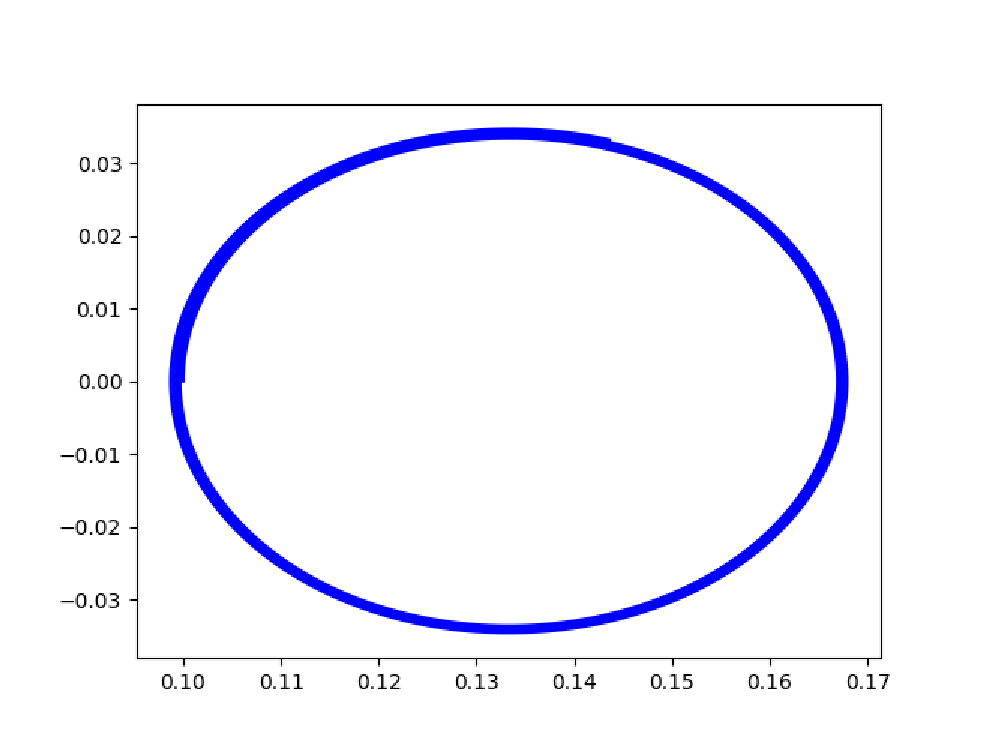
\includegraphics[scale=0.8]{./img/ka8_b3.eps}
\caption{$B=3$}
\label{8b3}
\end{figure}

\begin{figure}[H]
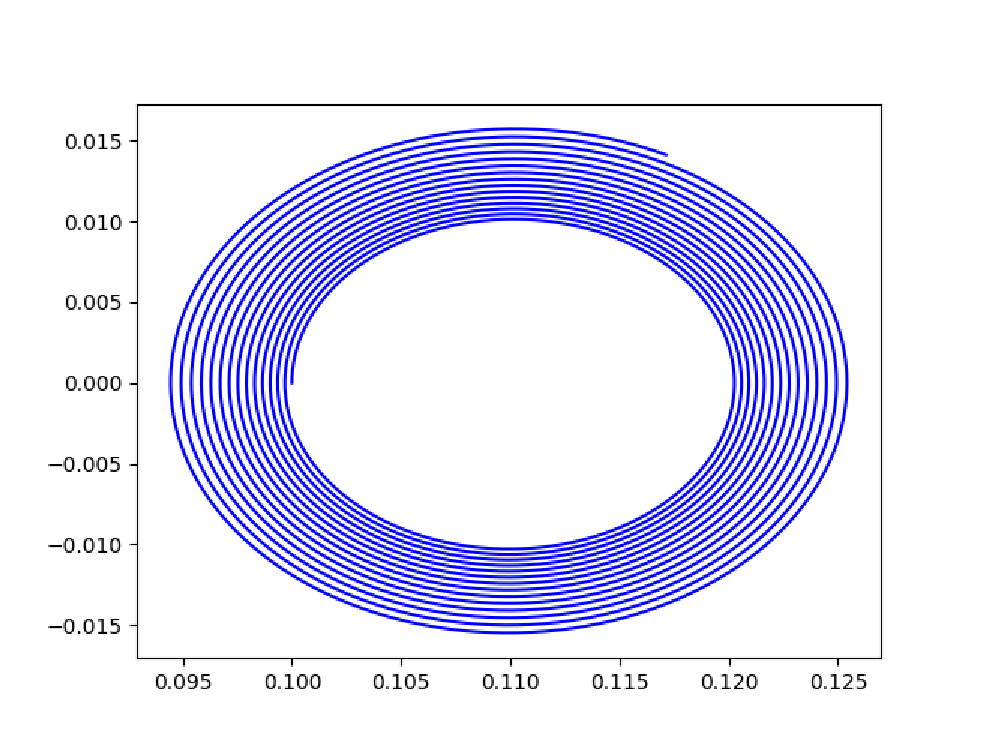
\includegraphics[scale=0.8]{./img/ka8_b10.eps}
\centering
\caption{$B=10$}
\label{8b10}
\end{figure}

誤差はそれぞれ次のようになった。

\begin{breakitembox}[l]{$B=1,3,10$のときの誤差}
    \begin{verbatim}
B: 1 ,誤差: 0.0092120809404796
B: 3 ,誤差: 0.08735045022264068
B: 10 ,誤差: 1.4792738717251592
 \end{verbatim}
\end{breakitembox}

$t=0の{v_x}^2+{v_y}^2$の値を $V_0$, $n$ステップ後の${v_x}^2+{v_y}^2$の値を$V_n$とすると、誤差は$(V_n - V_0)/V_0$で求められる.
$B$が大きくなればなるほど誤差が大きくなっており。エネルギー保存則が成り立たなくなっていることがわかる。
図\ref{8b1}--\ref{8b10}からも$B$が大きくなればなるほどエネルギー保存則が成り立たなくなり、より外側に軌道を描くようになっていることがわかる。
さらに、$B$が大きいほど円軌道が小さくなっており、$B$と円軌道の大きさは反比例の関係にあると考えられる。


\section{課題10 : ローレンツ力と電場}
課題9に電場から受ける力を追加し、ホイン法で解くプログラムを作成する。

\subsection{プログラムリスト}
課題10のプログラムリストをリスト\ref{lst:kadai10}に示す。

\lstinputlisting[style=C,caption=課題10のプログラム,label=lst:kadai10]{code/kadai10-2.c}

\subsection{実行結果}
課題10の実行結果をリスト\ref{lst:kekka10}に示す。

\begin{lstlisting}[style=text,caption=課題10の実行結果,label=lst:kekka10]
t = 0.00, x = (0.100000, 0.000000, 0.000000), v = (1.000000, 0.100000, 1.000000)
t = 0.01, x = (0.110050, 0.001005, 0.010050), v = (1.001005, 0.090050, 1.010050)
t = 0.02, x = (0.120110, 0.001910, 0.020201), v = (1.001910, 0.080090, 1.020201)
t = 0.03, x = (0.130179, 0.002715, 0.030454), v = (1.002715, 0.070121, 1.030454)
t = 0.04, x = (0.140257, 0.003420, 0.040810), v = (1.003420, 0.060144, 1.040810)
t = 0.05, x = (0.150341, 0.004024, 0.051270), v = (1.004024, 0.050160, 1.051270)
t = 0.06, x = (0.160431, 0.004528, 0.061835), v = (1.004528, 0.040170, 1.061835)
t = 0.07, x = (0.170527, 0.004932, 0.072507), v = (1.004932, 0.030175, 1.072507)
t = 0.08, x = (0.180626, 0.005235, 0.083286), v = (1.005235, 0.020176, 1.083286)
t = 0.09, x = (0.190729, 0.005438, 0.094173), v = (1.005438, 0.010174, 1.094173)
t = 0.10, x = (0.200834, 0.005540, 0.105169), v = (1.005540, 0.000170, 1.105169)
t = 0.11, x = (0.210939, 0.005542, 0.116276), v = (1.005542, -0.009836, 1.116276)
t = 0.12, x = (0.221045, 0.005443, 0.127495), v = (1.005443, -0.019841, 1.127495)
t = 0.13, x = (0.231150, 0.005244, 0.138826), v = (1.005244, -0.029845, 1.138826)
t = 0.14, x = (0.241253, 0.004944, 0.150271), v = (1.004944, -0.039847, 1.150271)
t = 0.15, x = (0.251352, 0.004543, 0.161831), v = (1.004543, -0.049846, 1.161831)
t = 0.16, x = (0.261448, 0.004042, 0.173508), v = (1.004042, -0.059841, 1.173508)
t = 0.17, x = (0.271538, 0.003441, 0.185302), v = (1.003441, -0.069832, 1.185302)
t = 0.18, x = (0.281623, 0.002739, 0.197214), v = (1.002739, -0.079816, 1.197214)
t = 0.19, x = (0.291701, 0.001937, 0.209246), v = (1.001937, -0.089793, 1.209246)
t = 0.20, x = (0.301770, 0.001034, 0.221399), v = (1.001034, -0.099762, 1.221399)
t = 0.21, x = (0.311830, 0.000032, 0.233674), v = (1.000032, -0.109723, 1.233674)
t = 0.22, x = (0.321881, -0.001071, 0.246072), v = (0.998929, -0.119673, 1.246072)
t = 0.23, x = (0.331920, -0.002274, 0.258595), v = (0.997726, -0.129612, 1.258595)
t = 0.24, x = (0.341947, -0.003576, 0.271244), v = (0.996424, -0.139540, 1.271244)
t = 0.25, x = (0.351961, -0.004979, 0.284020), v = (0.995021, -0.149454, 1.284020)
t = 0.26, x = (0.361961, -0.006481, 0.296925), v = (0.993519, -0.159355, 1.296925)
t = 0.27, x = (0.371946, -0.008082, 0.309959), v = (0.991918, -0.169240, 1.309959)
t = 0.28, x = (0.381915, -0.009783, 0.323124), v = (0.990217, -0.179110, 1.323124)
t = 0.29, x = (0.391867, -0.011583, 0.336421), v = (0.988417, -0.188962, 1.336421)
t = 0.30, x = (0.401800, -0.013482, 0.349852), v = (0.986518, -0.198797, 1.349852)
t = 0.31, x = (0.411715, -0.015480, 0.363418), v = (0.984520, -0.208613, 1.363418)
t = 0.32, x = (0.421609, -0.017577, 0.377120), v = (0.982423, -0.218409, 1.377120)
t = 0.33, x = (0.431482, -0.019772, 0.390961), v = (0.980228, -0.228184, 1.390961)
t = 0.34, x = (0.441334, -0.022065, 0.404940), v = (0.977935, -0.237937, 1.404940)
t = 0.35, x = (0.451162, -0.024456, 0.419059), v = (0.975544, -0.247668, 1.419059)
t = 0.36, x = (0.460966, -0.026945, 0.433321), v = (0.973055, -0.257374, 1.433321)
t = 0.37, x = (0.470745, -0.029532, 0.447726), v = (0.970468, -0.267056, 1.447726)
t = 0.38, x = (0.480499, -0.032216, 0.462275), v = (0.967784, -0.276712, 1.462275)
t = 0.39, x = (0.490225, -0.034997, 0.476971), v = (0.965003, -0.286342, 1.476971)
t = 0.40, x = (0.499923, -0.037874, 0.491815), v = (0.962126, -0.295944, 1.491815)
t = 0.41, x = (0.509592, -0.040849, 0.506808), v = (0.959151, -0.305517, 1.506808)
t = 0.42, x = (0.519232, -0.043919, 0.521951), v = (0.956081, -0.315060, 1.521951)
t = 0.43, x = (0.528841, -0.047085, 0.537247), v = (0.952915, -0.324573, 1.537247)
t = 0.44, x = (0.538417, -0.050347, 0.552696), v = (0.949653, -0.334055, 1.552696)
t = 0.45, x = (0.547961, -0.053705, 0.568301), v = (0.946295, -0.343504, 1.568301)
t = 0.46, x = (0.557472, -0.057157, 0.584062), v = (0.942843, -0.352920, 1.584062)
t = 0.47, x = (0.566947, -0.060704, 0.599982), v = (0.939296, -0.362301, 1.599982)
t = 0.48, x = (0.576387, -0.064345, 0.616062), v = (0.935655, -0.371647, 1.616062)
t = 0.49, x = (0.585790, -0.068080, 0.632303), v = (0.931920, -0.380957, 1.632303)
t = 0.50, x = (0.595156, -0.071908, 0.648708), v = (0.928092, -0.390229, 1.648708)
t = 0.51, x = (0.604484, -0.075830, 0.665277), v = (0.924170, -0.399464, 1.665277)
t = 0.52, x = (0.613771, -0.079845, 0.682013), v = (0.920155, -0.408659, 1.682013)
t = 0.53, x = (0.623019, -0.083952, 0.698917), v = (0.916048, -0.417815, 1.698917)
t = 0.54, x = (0.632225, -0.088151, 0.715992), v = (0.911849, -0.426930, 1.715992)
t = 0.55, x = (0.641389, -0.092442, 0.733237), v = (0.907558, -0.436002, 1.733237)
t = 0.56, x = (0.650510, -0.096823, 0.750656), v = (0.903177, -0.445033, 1.750656)
t = 0.57, x = (0.659587, -0.101296, 0.768250), v = (0.898704, -0.454019, 1.768250)
t = 0.58, x = (0.668619, -0.105859, 0.786021), v = (0.894141, -0.462961, 1.786021)
t = 0.59, x = (0.677605, -0.110512, 0.803971), v = (0.889488, -0.471858, 1.803971)
t = 0.60, x = (0.686545, -0.115254, 0.822101), v = (0.884746, -0.480708, 1.822101)
t = 0.61, x = (0.695436, -0.120085, 0.840413), v = (0.879915, -0.489512, 1.840413)
t = 0.62, x = (0.704280, -0.125005, 0.858909), v = (0.874995, -0.498267, 1.858909)
t = 0.63, x = (0.713073, -0.130012, 0.877591), v = (0.869988, -0.506973, 1.877591)
t = 0.64, x = (0.721817, -0.135107, 0.896461), v = (0.864893, -0.515629, 1.896461)
t = 0.65, x = (0.730509, -0.140289, 0.915520), v = (0.859711, -0.524235, 1.915520)
t = 0.66, x = (0.739149, -0.145558, 0.934771), v = (0.854442, -0.532789, 1.934771)
t = 0.67, x = (0.747736, -0.150912, 0.954216), v = (0.849088, -0.541291, 1.954216)
t = 0.68, x = (0.756269, -0.156352, 0.973856), v = (0.843648, -0.549739, 1.973856)
t = 0.69, x = (0.764748, -0.161877, 0.993693), v = (0.838123, -0.558134, 1.993693)
t = 0.70, x = (0.773171, -0.167486, 1.013729), v = (0.832514, -0.566473, 2.013729)
t = 0.71, x = (0.781538, -0.173179, 1.033967), v = (0.826821, -0.574756, 2.033967)
t = 0.72, x = (0.789847, -0.178956, 1.054409), v = (0.821044, -0.582983, 2.054409)
t = 0.73, x = (0.798099, -0.184815, 1.075056), v = (0.815185, -0.591153, 2.075056)
t = 0.74, x = (0.806292, -0.190756, 1.095910), v = (0.809244, -0.599264, 2.095910)
t = 0.75, x = (0.814424, -0.196778, 1.116974), v = (0.803222, -0.607316, 2.116974)
t = 0.76, x = (0.822497, -0.202882, 1.138249), v = (0.797118, -0.615308, 2.138249)
t = 0.77, x = (0.830508, -0.209066, 1.159739), v = (0.790934, -0.623239, 2.159739)
t = 0.78, x = (0.838457, -0.215329, 1.181444), v = (0.784671, -0.631109, 2.181444)
t = 0.79, x = (0.846343, -0.221672, 1.203368), v = (0.778328, -0.638916, 2.203368)
t = 0.80, x = (0.854165, -0.228093, 1.225511), v = (0.771907, -0.646661, 2.225511)
t = 0.81, x = (0.861923, -0.234592, 1.247878), v = (0.765408, -0.654341, 2.247878)
t = 0.82, x = (0.869615, -0.241168, 1.270469), v = (0.758832, -0.661957, 2.270469)
t = 0.83, x = (0.877241, -0.247821, 1.293287), v = (0.752179, -0.669507, 2.293287)
t = 0.84, x = (0.884801, -0.254549, 1.316335), v = (0.745451, -0.676992, 2.316335)
t = 0.85, x = (0.892292, -0.261353, 1.339614), v = (0.738647, -0.684409, 2.339614)
t = 0.86, x = (0.899716, -0.268232, 1.363127), v = (0.731768, -0.691758, 2.363127)
t = 0.87, x = (0.907070, -0.275184, 1.386877), v = (0.724816, -0.699040, 2.386877)
t = 0.88, x = (0.914354, -0.282209, 1.410865), v = (0.717791, -0.706251, 2.410865)
t = 0.89, x = (0.921568, -0.289307, 1.435094), v = (0.710693, -0.713393, 2.435094)
t = 0.90, x = (0.928711, -0.296476, 1.459566), v = (0.703524, -0.720465, 2.459566)
t = 0.91, x = (0.935781, -0.303717, 1.484285), v = (0.696283, -0.727465, 2.484285)
t = 0.92, x = (0.942779, -0.311028, 1.509252), v = (0.688972, -0.734393, 2.509252)
t = 0.93, x = (0.949703, -0.318409, 1.534470), v = (0.681591, -0.741248, 2.534470)
t = 0.94, x = (0.956553, -0.325858, 1.559942), v = (0.674142, -0.748030, 2.559942)
t = 0.95, x = (0.963328, -0.333376, 1.585669), v = (0.666624, -0.754738, 2.585669)
t = 0.96, x = (0.970028, -0.340961, 1.611655), v = (0.659039, -0.761371, 2.611655)
t = 0.97, x = (0.976651, -0.348613, 1.637902), v = (0.651387, -0.767928, 2.637902)
t = 0.98, x = (0.983197, -0.356331, 1.664413), v = (0.643669, -0.774409, 2.664413)
t = 0.99, x = (0.989666, -0.364113, 1.691190), v = (0.635887, -0.780814, 2.691190)
t = 1.00, x = (0.996057, -0.371961, 1.718237), v = (0.628039, -0.787141, 2.718237)
\end{lstlisting}

\subsection{考察}
$B=E=1.0$, $B=1.0, E=2.0$, $B=0.5, E=1.0$のときの実行結果をグラフにプロットしたものを、
図\ref{fig:1}, \ref{fig:2}, \ref{fig:3}に示す。
図\ref{fig:2}を見ると、\ref{fig:1}に比べて、$z$軸方向への加速度が大きいことが分かる。
図\ref{fig:3}を見ると、\ref{fig:1}に比べて、円運動の半径は大きく、$z$軸方向への加速度は小さいことが分かる。


\begin{figure}[H]
  \centering
  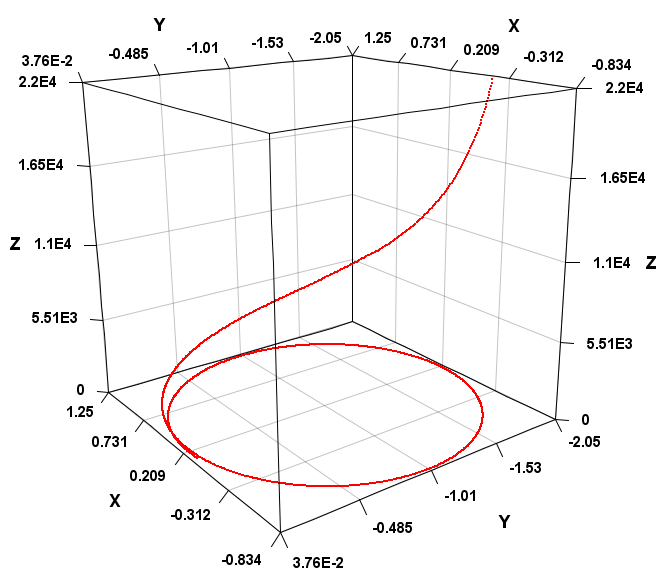
\includegraphics[width=12cm]{1.png}
  \caption{$B=E=1.0$}
  \label{fig:1}
\end{figure}

\begin{figure}[H]
  \centering
  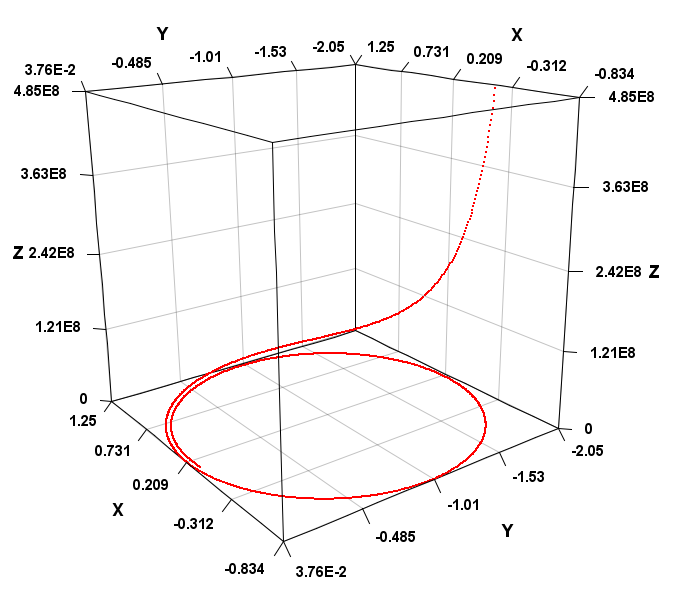
\includegraphics[width=12cm]{2.png}
  \caption{$B=1.0, E=2.0$}
  \label{fig:2}
\end{figure}

\begin{figure}[H]
  \centering
  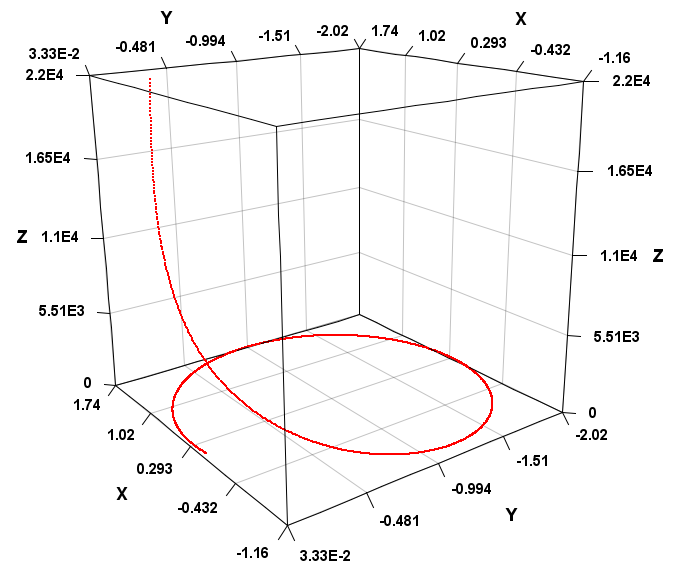
\includegraphics[width=12cm]{3.png}
  \caption{$B=0.5, E=1.0$}
  \label{fig:3}
\end{figure}


\end{document}
